\chapter{Single-Cell Omics: State of the Art}
\label{ch:litrev}
All life originates from and operates as a massive, interconnected network of molecules. The term 'omics' refers to the systematic characterisation of these elements in order to elucidate their relation to development, function and disease. Since the advent of genomics in the mid 90s shortly after the first genomes of small organisms were sequenced, several new 'omics' fields have emerged. Transcriptomics focuses on the quantification and characterisation of all \acrshort{rna} transcripts. Epigenomics revolves around chromatin changes and their relation to gene expression. Since the focus of omics is a complete overview of an entire class of molecules, the availability of high-throughput analysis methods is critical in these fields \citep{hood2004, patti2012, patterson2003}\pms

Since the mid 2000s, several bulk omics analysis techniques have allowed researchers to explore the complete transcriptomes and epigenomes of pre-defined cell populations. These techniques often require explicit cell pre-selection, for example using \acrfull{facs} and established marker genes. In the bulk approach, the sampled population is isolated as a group and further treated as a single, homogeneous entity. Any information on heterogeneity within that population is disregarded, masking the presence of previously undiscovered and rare cell types \citep{bengtsson2005, wang2010, kolodziejczyk2015, grun2015}.\pms

For decades, however, researchers have acknowledged that morphologically homogeneous cells may exhibit vastly different transcriptional profiles. One of the earliest mentions of this idea occurred in \citeyear{eberwine1992}, when \citeauthor{eberwine1992} discovered that in a sample of 15 rat hippocampus pyramidal cells, 2 cells exhibited significantly different \acrfull{mrna} profiles than the rest of the population \citep{eberwine1992}. Realising the power of their discovery, the authors suggested that analysing single cells could help identify new cell types, reveal gene transcript subtypes and even directly determine the influence of external stimuli on a cell's gene expression. However, the single-cell analysis methods employed by \citeauthor{eberwine1992} were expensive and laborious, prohibiting large-scale application of the technique. Indeed, the challenges associated with analysing single cells are numerous and complex:

\begin{enumerate}
	\setlength{\itemsep}{0pt}%
	\setlength{\parskip}{0pt}%
	\item Single cells need to be isolated from complex tissue matrices while preserving their natural state as closely as possible.
	\item The minute nucleic acid content of single cells (\SI{}{\pico\gram}) calls for sensitive library generation protocols before sequencing can occur. This problem is exacerbated by the relative \acrshort{mrna} transcript levels of different genes, which can span orders of magnitudes between and within single cells from the same tissue \citep{bengtsson2005}.
	\item Due to the large number of cells, the aforementioned challenges need to be tackled in ways that permit high throughput and low reaction volumes to reduce time, cost and labour while maintaining sufficient efficiency and sensitivity.
\end{enumerate}

In the past few years, technological progress in microfluidics and next-generation sequencing have enabled researchers to overcome many of these challenges. Using advanced separation techniques, single cells can now be isolated and analysed individually with increasing accuracy. Ultra-sensitive amplification techniques and transcript barcoding allow sequencing of a single cell's \acrshort{dna} or \acrshort{mrna} content. Since these single-cell sequencing techniques are usually dependent only on basic reagents and machinery, many research institutes have started to adopt them, leading to a rapid increase in the number of publications using them (figure \ref{fig:evolution}).

\begin{figure}[ht]
	\centerfloat
	\def\svgwidth{14cm}
	\input{./ims/evolution.pdf_tex}
	\caption[Number of publications in single-cell omics]{Number of abstracts published in scientific journals containing the words "single-cell" and "sequencing". Data gathered from Scopus.}
	\label{fig:evolution}
\end{figure}

%todo[inline]{spice this image up with some key timepoints, first microfluidics and whatnot}

Single-cell analysis techniques have been used to uncover transcriptional heterogeneity in tissues previously deemed homogeneous, to identify new transcripts, map cell state trajectories in (pseudo)time, to study the effect of gene knockdowns and to unravel gene regulatory networks \citep{tang2011}.\pms

In this literature study, the current state of the art in single-cell research is examined. First, a selection of popular single-cell analysis techniques is explained using their cell separation strategy as a basic classification criterion. Figure \ref{fig:stuart2019} shows the general subdivision of the reviewed methods. We start with the most straightforward approach: applying established bulk analysis methods on single-cells sorted in microwells. Then, two techniques that automatically load cells into microfluidic arrays in order to decrease labour are discussed. Third, we look at how droplet microfluidics lead to a 100-fold increase in cell throughput. Fourth, a number of ultra-high throughput well-based protocols is discussed briefly. After the state of the art is established, we go over some of the most important breakthroughs in biology fueled by single-cell research. Finally, a short conclusion is drawn on single-cell research and possible future perspectives of single-cell omics are posed.\pms

\begin{figure}[ht]
	\centerfloat
	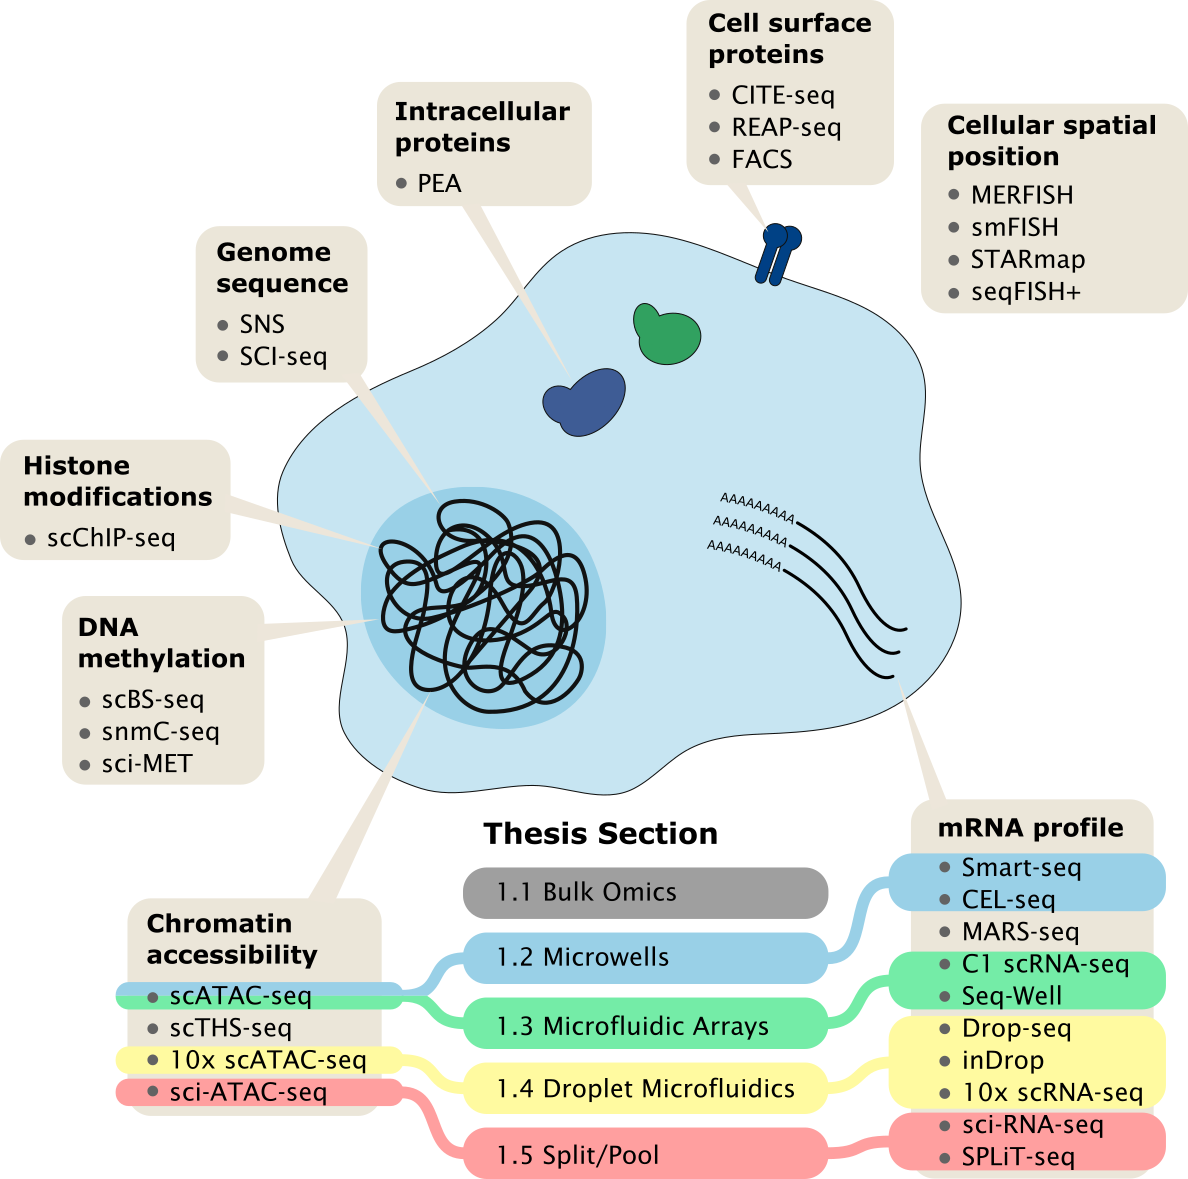
\includegraphics[width=12cm]{./ims/stuart2019.png}
	\caption[Current single-cell technology landscape]{\textbf{Current single-cell technology landscape.} An array of analysis techniques can be used to study genomics, transcriptomics, proteomics and epigenomics at single-cell resolution. In this literature study, a number of important single-cell techniques are explained and compared. Modelled after \cite{stuart2019}.}
	\label{fig:stuart2019}
\end{figure}

%\input{./tex/lit_tree}

\newpage
\section{Bulk Omics Techniques}
\label{sec:lit_bulk}
Before single-cell analysis techniques can be discussed, the bulk techniques which they are founded on need to be thoroughly understood. The following section will briefly explain \acrshort{rna-seq} and \acrshort{atac-seq}, which have both become a major point of focus in the single-cell omics landscape and will play a key role in the experimental part of this work.\pms

\subsection{RNA-seq}
\label{subsect:lit_rna-seq}
The transcriptome comprises all \acrshort{mrna} transcripts, the functional elements of the genome, in a cell population. Transcriptomics focuses on the quantification of these \acrshort{mrna} transcripts and how their levels change during disease and development. Previous generations of transcriptomic techniques, such as expression microarrays, suffer from hybridisation artefacts, cannot detect splice variants or new genes, have a low dynamic range and yield semi-quantitative data due to the limitations of fluorescence \citep{wang2009, tang2011}. \acrshort{rna-seq}, first described in \citeyear{mortazavi2008}, was the first comprehensive and simple protocol to offer accurate quantification of a cell population's gene expression without requiring cloning of the sample \acrshort{rna} \citep{mortazavi2008}.\pms

\acrshort{rna-seq} evades the pitfalls of hybridisation and fluorescence-dependent methods by sequencing the \acrshort{cdna} of captured \acrshort{mrna} (fig. \ref{fig:wang2009}). By using oligo(dT) magnetic beads to capture poly-A tails (repetitions of adenosine nucleotides that is incorporated in all mature \acrshort{mrna} transcripts), transcripts can be detected without explicit previous knowledge of their sequence. In the next step, fragmentation of the captured \acrshort{mrna} destroys secondary structures and mitigates transcript length variation, improving upon random hexamer reverse transcription priming. Optionally, Arabidopsis and phage lambda \acrshort{rna} standards can be co-processed with the sample in order to allow absolute transcript quantification. These known \acrshort{rna} sequences are added at set concentrations, yielding a linear standard curve which can be used to relate read count and transcript concentration. In the 140 million reads generated by \acrshort{rna-seq}, \citeauthor{mortazavi2008} detected alternative splice variants for 3 462 genes and identified 596 new candidate transcripts in mouse brain, liver and muscle.\pms

\begin{figure}[ht]
	\centerfloat
	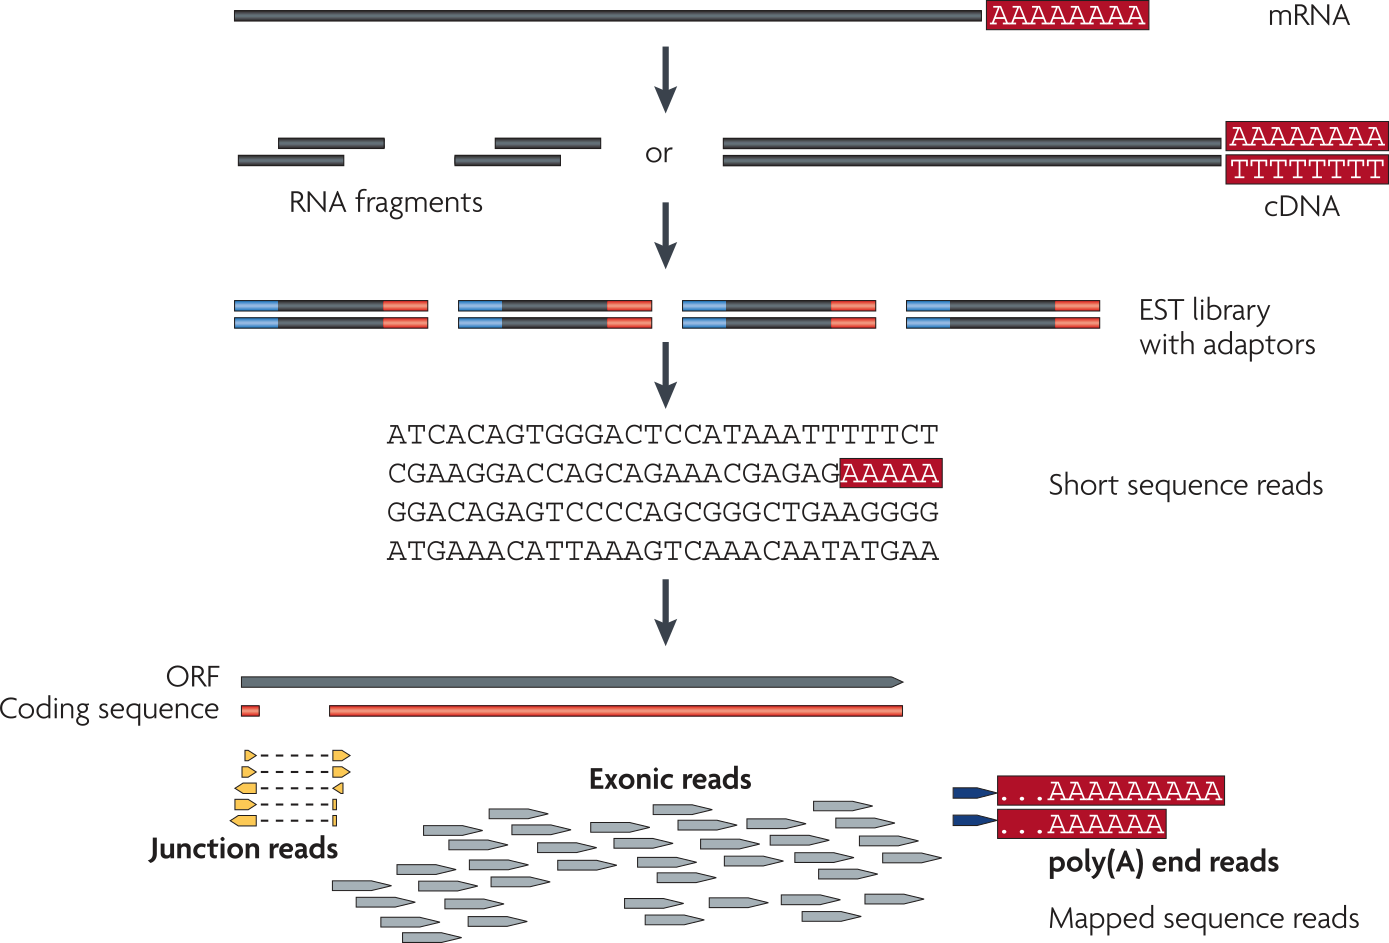
\includegraphics[width=\textwidth]{./ims/wang2009.png}
	\caption[RNA-seq workflow]{\textbf{RNA-seq workflow.} Processed \acrshort{mrna} transcripts are captured using poly-T magnetic beads and hydrolised to 200-300 \acrshort{bp} fragments to remove secondary structures. After reverse transcription using random hexamer primers and second strand synthesis, the fragments are processed into a sequencing library. Sequencing and alignment to a reference transcriptome or exome yields an accurate overview of the sample tissue's expression profile. Additionally, clusters of reads that do not map to previously known exons can be organised into candidate exons in order to identify newly transcribed regions. Adapted from \citealt{wang2009}}
	\label{fig:wang2009}
\end{figure}

\acrshort{rna-seq} offers uniform transcript coverage, accurate quantification of transcripts up to 1 transcript/cell, a dynamic quantification range of five orders of magnitude, and is able to detect transcripts outside of the prior reference transcriptome. Generated data is highly replicable and correlates well to \acrshort{rna}-microarray data. \acrshort{rna-seq} allows researchers to detect differences in transcriptional profile in response to certain conditions or along development, to catalogue different species of transcripts and to determine the transcriptional structure of genes. Due to its simplicity and low cost, \acrshort{rna-seq} remains one of the main techniques used in transcriptomics to date. However, the method is still sensitive to strongly related sequences in the exome such as gene duplications and paralogs \citep{wang2009}. In \citeyear{kivioja2012}, a method for absolute transcript quantification was developed \citep{kivioja2012}. Here, each reverse transcription primer carries a sequence of 10 additional random nucleotides, called the \acrfull{umi}. This \acrshort{umi} is incorporated into each \acrshort{cdna} transcript. After \acrshort{pcr}, each amplification product can now be traced back to its transcript of origin by its \acrshort{umi}, allowing absolute quantification of the original number of transcripts present in the sample.\pms

\newpage
\subsection{ATAC-seq}
\label{subsect:lit_atac-seq}
The \acrshort{dna} of eukaryotic cells is organised into chromatin, an organised complex of nucleic acid and histone nucleoproteins. This form of compaction allows the cell's entire genome to fit into the nuclear subspace \citep{kornberg1974}. When \acrshort{dna} is packed tightly around these nucleoproteins, the underlying genes sequences are inaccessible to transcription factors, inhibiting transcription of the restricted \acrshort{dna}. However, using an array of mechanisms such as \acrshort{dna} methylation, nucleosome positioning and histone modification, the cell can locally remodel the steric accessibility of chromatin to allow gene transcription. Chromatin accessibility state is therefore a leading indicator of which genes are actively expressed in a cell and, together with \acrshort{dna} methylation and histone modification, forms the physical basis of epigenomics \citep{jaenisch2003, kouzarides2007, schones2008, bannister2011}. Epigenomic variation has been shown to be highly variable in time, between cell populations and across cell generations and thus effectively provides a layer of information "on top of" the cell's genome. Studying epigenomic phenomena can thus help construct models of gene regulatory pathways. A thorough understanding of these pathways may ultimately help answer the question of how different cell phenotypes can arise from genetically identical precursor cells \citep{johannes2008}.\pms

The chromatin state of cell populations has previously been studied using techniques such as \acrshort{faire-seq} and \acrshort{dnase-seq}  \citep{giresi2007, song2010, gaulton2010, song2011}. However, these methods involve steps such as chloroform extraction and gel purification which may lead to loss of sensitivity. The \acrfull{atac-seq}, a technique published by \citeauthor{buenrostro2013} in \citeyear{buenrostro2013}, allows researchers to investigate the chromatin condensation state of a cell population without such potentially loss-prone steps. \acrshort{atac-seq} relies on the activity of a hyperactive, mutated Tn5 transposase which (near)-randomly fragments only sterically accessible chromatin regions. In contrast to DNase, another enzyme that randomly fragments accessible chromatin, Tn5 ligates oligonucleotide adapters where it cleaves \acrshort{dna}. Strands fragmented by Tn5 are thus flanked by two adapter sequences. These adapters can then be used in \acrshort{pcr} as hybridisation sites for specialised sequencing primers, simplifying post-fragmentation processing (fig. \ref{fig:atacseq}).\pms

\begin{figure}
	\begin{minipage}[]{0.6\textwidth}
		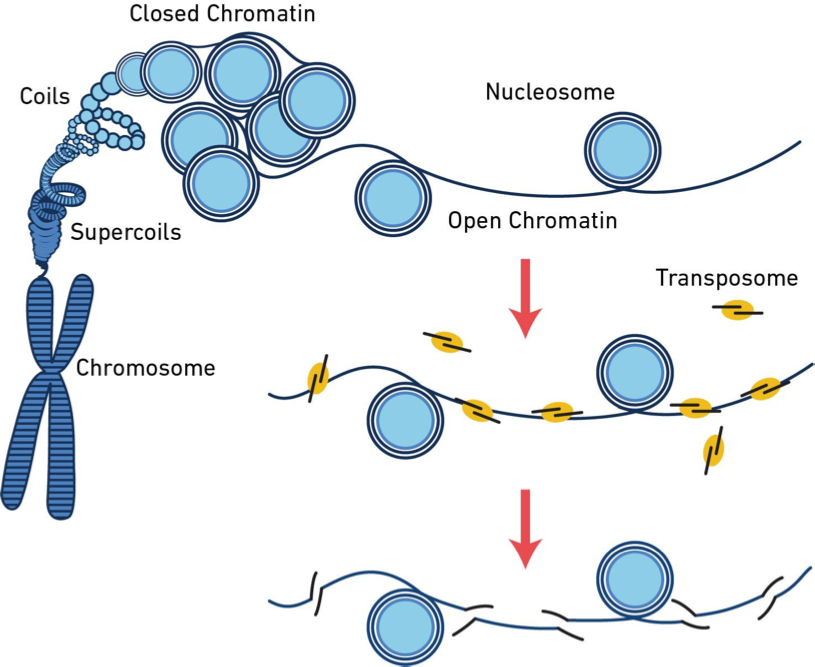
\includegraphics[width=\textwidth]{./ims/atacseq.png}
	\end{minipage}\hfill
	\begin{minipage}[]{0.35\textwidth}
		\captionsetup{margin={18pt,0pt}, labelfont=bf}
		\caption[ATAC-seq concept]{\textbf{\acrshort{atac-seq} concept.} Tn5 transposase fragments \acrshort{dna} only in sterically accessible chromatin and ligates adapters. A subsequent \acrshort{pcr} uses these adapters to incorporate sequencing adapters and sample indexes. After sequencing, reads are mapped to a reference. Source: 10x Cell Ranger ATAC Algorithm brochure}
		\label{fig:atacseq}
	\end{minipage}
\end{figure}

Random fragmentation of accessible \acrshort{dna} results in many short fragments of the accessible chromatin and fewer but longer fragments of the inaccessible regions. The fragment length and count can therefore be used to determine the "accessibility" of a given chromatin region. Areas of significant enrichment in the read distribution are detected computationally in a process called peak calling, yielding information on which regions of the genome are accessible in the cell population.\pms

% \todo[inline]{put a bunch of sources here, or keep for later in the section where important results are shown. ref to applicatioins?}

\acrshort{atac-seq} requires a starting number of cells 2 - 3 orders of magnitude lower than \acrshort{dnase-seq}  and \acrshort{faire-seq} ({\textasciitilde}50 000 versus {\textasciitilde}50 000 000). The protocol takes only {\textasciitilde}5 hours from sample collection to sequencing compared to 3.5 days for \acrshort{dnase-seq}, but the resulting data is of similar quality \citep{buenrostro2013}. In \citeyear{corces2017}, a more widely-applicable bulk \acrshort{atac-seq} protocol, dubbed "Omni-\acrshort{atac-seq}", was released. This updated version is applicable to a broader range of cell types and yields a higher fraction of reads in peaks than the standard \acrshort{atac-seq}. Importantly, the improved protocol also efficiently removes mitochondrial \acrshort{dna} from the transposition reaction, hereby reducing sequencing costs \citep{corces2017}. As will be shown later, recent efforts have scaled ATAC-seq up to single-cell resolution \citep{buenrostro2015, chen2018}.\pms

\newpage
\section{Microwell-based Single-Cell Omics Techniques}
\label{sec:lit_well-based}
Some of the earliest efforts to analyse the nucleic acid content of single cells simply applied bulk analysis techniques to single cell lysate suspended in small compartments. For example, \citeauthor{eberwine1992} carried out reverse transcription of \acrshort{mrna} by injecting a live cell with viral reverse transcriptase and oligo-dT primers and aspirating the cell contents into the glass electrode. Due to the high fixed labour cost and limits of technology at the time, their approach led to extremely low throughput compared to today's standard: 5 days of work for 1 cell then, compared to 5 days of work for 10 000 cells today \citep{hashimshony2012}. The following section shows recent continuations on the microcompartment approach, which have become widespread due to their ease of use.\pms

\subsection{Smart-seq}
\label{subsect:lit_smart-seq}
\Acrfull{smart-seq}, originally formulated by \citeauthor{ramskold2012} in \citeyear{ramskold2012}, was one of the first single-cell \acrshort{mrna}-seq protocols and the first to provide full transcript coverage. The technique is modelled after an earlier \acrshort{mrna}-seq protocol by \cite{tang2009}, who sequenced the transcriptome of a single mouse blastomere.\pms

\citeauthor{ramskold2012} first applied \acrshort{smart-seq} to 42 human cells manually picked from dissociated tissues using microscope-assisted micromanipulation. Single cells were further treated separately in microwells. Figure \ref{fig:ramskold2012} shows the steps involved in \acrshort{smart-seq} library generation. An important addition of \acrshort{smart-seq} compared to the \citeauthor{tang2009} protocol is the use of template switching. During reverse transcription, the \acrfull{mmlv} reverse transcriptase adds extra cytosines to the 3' end of the \acrshort{cdna} strand, allowing a so-called \acrfull{tso} to hybridise. \acrshort{mmlv} reverse transcriptase then continues \acrshort{cdna} synthesis using the \acrshort{tso} as a template in a process called template switching. The sequence complementary to the \acrshort{tso} is thus incorporated in the \acrshort{cdna} library and is used as a \acrshort{pcr} priming site in further amplification steps. Importantly, the SMART primer can hybridise to both ends of the \acrshort{cdna} transcript. The \acrshort{pcr} product of short templates can thus form loops which impede further amplification. This mechanism corrects the natural short-fragment bias associated with \acrshort{pcr} amplification. The template-switching reverse transcription approach is more user-friendly and time-efficient than linear amplification by in-vitro transcription. Compared to a regular reverse transcription, template-switching also produces \acrshort{cdna} transcripts of the complete \acrshort{rna} template. This means that any splicing information carried by the very distal ends of the transcript is retained after sequencing.\pms

\begin{figure}[ht]
	\centerfloat
	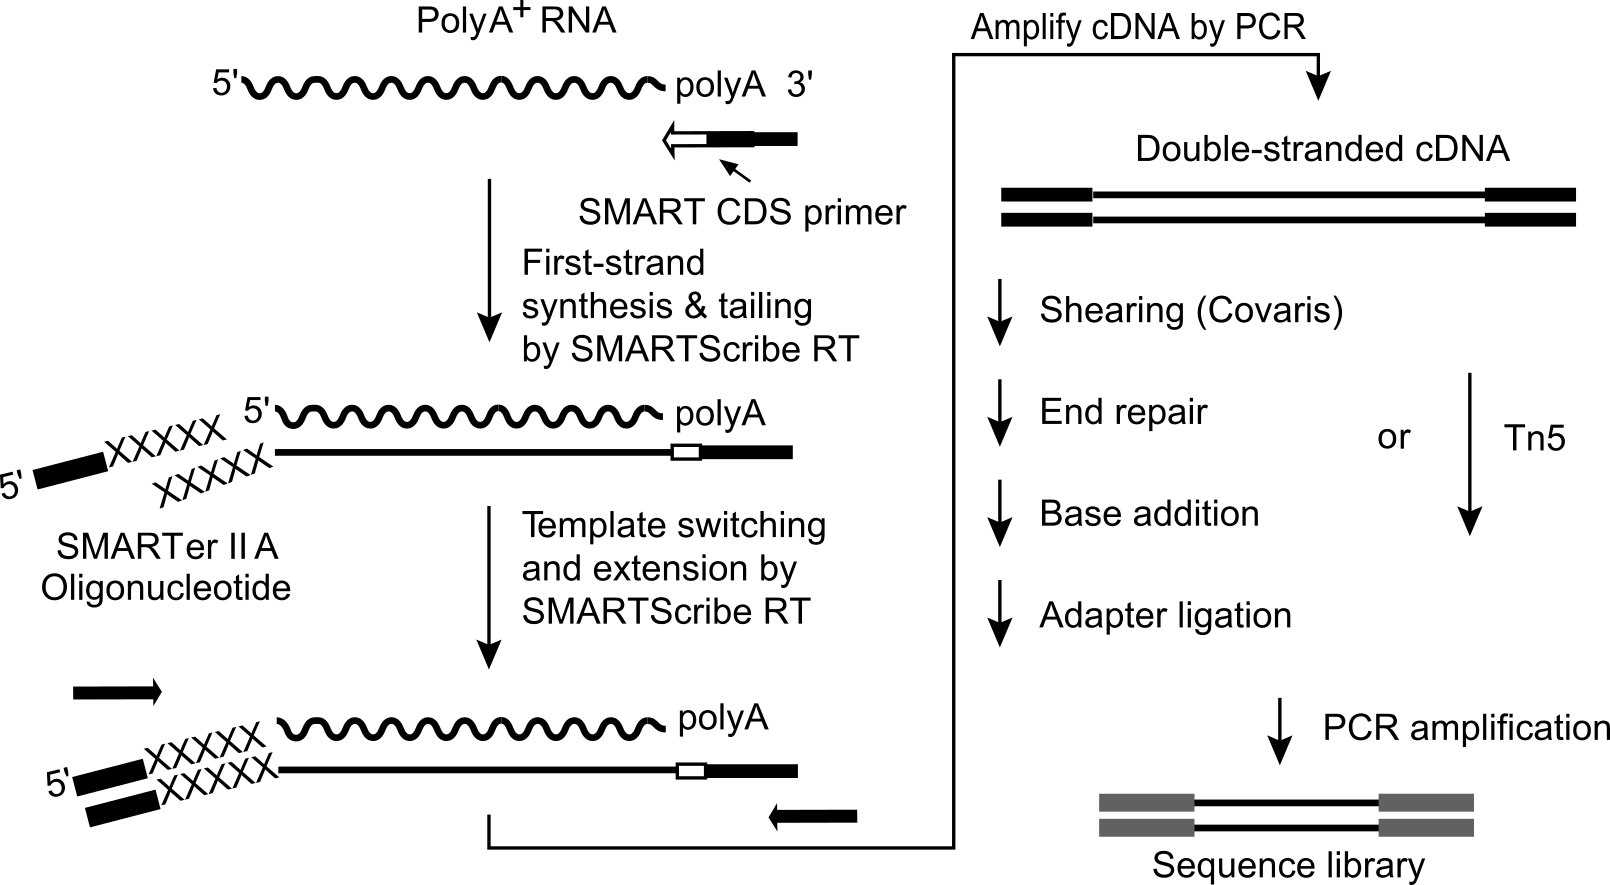
\includegraphics[width=\textwidth]{./ims/ramskold2012.png}
	\caption[Smart-seq library generation]{\textbf{Smart-seq library generation.} Single cells are manually isolated from dissociated sample tissue and placed in separate microwells. The cells are then lysed and their polyadenylated \acrshort{mrna} content is captured by oligo(dT) reverse transcription primers. Full transcript \acrshort{cdna} is synthesised using \acrshort{mmlv} reverse transcriptase and pre-amplified by \acrshort{ispcr}. Double-stranded \acrshort{cdna} is then fragmented and tagged with sequencing primers and adapters by Tn5. Alternatively, shearing and adapter ligation can be used. After further \acrshort{pcr} amplification, the library is ready for next-generation sequencing. Adapted from \citealp{ramskold2012}.}
	\label{fig:ramskold2012}
\end{figure}

An improvement on \acrshort{smart-seq}, \acrshort{smart-seq}2, was published by \citeauthor{picelli2013} in \citeyear{picelli2013}. Here, single cell isolation was performed on 262 human and mouse cells. In the improved \acrshort{smart-seq}2 protocol, \acrshort{cdna}-yield was increased twofold by incorporating a \acrfull{lna} in the \acrshort{tso}. This small change led to better thermal stability of the \acrshort{tso}-\acrshort{cdna} duplex. Further reagent concentration optimisations resulted in an overall increase in sensitivity and accuracy relative to \acrshort{smart-seq}. \citeauthor{picelli2013} report that \acrshort{smart-seq}2 detects \textasciitilde{}12k genes from \acrshort{hek} cells compared to \textasciitilde{10k} genes detected by first generation \acrshort{smart-seq}. Additionally, cells were isolated by distributing \SI{}{\micro\litre} volumes of strongly diluted cell suspensions into microwells instead of relying on manual cell picking. This allows for the use of automated liquid handling, but incurs an additional increase in reagent cost due to empty wells. An overview of the \acrshort{smart-seq}2 library generation workflow is given in figure \ref{fig:picelli2014_fig1_edited}.\pms

\begin{figure}
	\centerfloat
	\def\svgwidth{\textwidth}
	\input{./ims/picelli2014_fig1_edited.pdf_tex}
	\caption[Smart-seq2 library generation]{\textbf{Smart-seq2 library generation.} Single cells from a dilute cell suspension are distributed into separate microwells. The cells are then lysed and their polyadenylated \acrshort{mrna} content is captured by oligo(dT) reverse transcription primers. After full-transcript reverse transcription by template switching using an \acrshort{lna}-\acrshort{tso}, the resulting \acrshort{cdna} is pre-amplified and subsequently tagmented with sequencing adapters using Tn5 transposase. The library is then further amplified and sequenced. Adapted from \citealp{picelli2014}.}
	\label{fig:picelli2014_fig1_edited}
\end{figure}

\Acrshort{smart-seq} and \acrshort{smart-seq}2 yield full transcript information and thus allow researchers to study both distal and proximal splicing events, novel exon detection, single-cell \acrshort{snp} detection, and allele-specific gene expression \citep{kolodziejczyk2015}. However, using microwells reduces throughput and increases reaction volumes, leading to an overall increased cost per cell. Cell selection based on dilution also inhibits the detection of rare cell types in large samples. The \acrshort{smart-seq} and \acrshort{smart-seq}2 protocols do not incorporate \acrshortpl{umi} into the \acrshort{cdna}, making absolute quantification of transcripts impossible. The use of double-stranded \acrshort{cdna} also discards information about transcript strand specificity. Moreover, the random fragmentation nature of the Tn5 tagmentation reaction leads to a reduced sequencing coverage of the very 5' ends of transcripts, which carry the \acrfull{tss} and \acrfull{5utr}. Studying these important regions is therefore difficult using \acrshort{smart-seq}. In conclusion, \acrshort{smart-seq}2 is a highly sensitive, but low-throughput method best suited for small cell populations where the complete \acrshort{mrna} transcript is needed to investigate distal splicing or presence of \acrshortpl{snp}. Since \acrshort{smart-seq}2 requires only off-the shelf reagents and equipment, it has become a widespread single-cell \acrshort{rna-seq} protocol \citep{picelli2017}.\pms

\newpage
\subsection{CEL-seq}
\label{subsect:lit_cel-seq}
\Acrfull{cel-seq}, published in \citeyear{hashimshony2012} by \citeauthor{hashimshony2012}, is a single-cell transcriptomics technique revolving around \acrshort{mrna} barcoding followed by \acrfull{ivt} for linear amplification. \Acrshort{ivt} leads to more reproducible and sensitive results compared to exponential \acrshort{pcr} amplification, but requires \textasciitilde\SI{400}{\pico\gram} of \acrshort{cdna} compared to the average eukaryotic cell's \acrshort{mrna} content of \textasciitilde\SI{1}{\pico\gram} \citep{tang2011, hashimshony2012}. \acrshort{cel-seq} satisfies this requirement by pooling barcoded \acrshort{cdna} from different cells of origin before applying \acrshort{ivt}. Due to the in vitro transcription step which generates only sense RNA from antisense \acrshort{cdna}, \acrshort{cel-seq} generates strand-specific sequencing libraries. For a detailed overview of the \acrshort{cel-seq} protocol, see \citep{hashimshony2012}. A second generation protocol, \acrshort{cel-seq}2, was published in \citeyear{hashimshony2016}. Figure \ref{fig:hashimshony2016_fig1_edited} shows the generalised \acrshort{cel-seq}2 workflow.\pms

\begin{figure}
	\centerfloat
	\def\svgwidth{\textwidth}
	\input{./ims/hashimshony2016_fig1_edited.pdf_tex}
	\caption[CEL-seq2 library generation]{\textbf{CEL-seq2 library generation.} Single cells are lysed and poly-A\textsuperscript{+} \acrshort{mrna} is reverse transcribed using a poly-T primer that includes a cell-specific barcode, a transcript-specific \acrshort{umi}, an Illumina 5' adapter and a T7 promoter. Pooled \acrshort{cdna} is transcribed in vitro and the amplified RNA is purified. Then, using a random primer with overhang complementary to the 3'-adapter, inserts flanked with a 3' Illumina sequencing adapter are generated which are then purified and processed for paired-end sequencing. Adapted from \cite{hashimshony2016}}
	\label{fig:hashimshony2016_fig1_edited}
\end{figure}

\acrshort{cel-seq}2 increases reverse transcription efficiency by shortening the reverse transcription primer. This leads to a higher fraction of \acrshort{mrna} transcripts being detected. Incorporating Illumina sequencing adapters during reverse transcription eliminates a \acrshort{pcr}-ligation step, increasing read mappability from 60.9\% to 93.8\%. \acrshort{cel-seq}2 also incorporates a \acrshort{umi} into every \acrshort{cdna} strand, enabling absolute transcript quantification. These incremental improvements together lead to a 30\% increase in number of genes detected compared to the first generation \acrshort{cel-seq}. It is also shown that \acrshort{cel-seq}2 can be readily performed on the Fluidigm C1 microfluidic platform for increased gene detection and reduced labour cost \citep{hashimshony2016}.\pms

Compared to \acrshort{smart-seq}, \acrshort{cel-seq}2 yields a near 100\% increase in genes detected on the same cell sample \citep{hashimshony2016}. \acrshort{cel-seq}2, however, is strongly 3'-biased and can therefore not provide information on distal splicing as opposed to \acrshort{smart-seq}. Importantly, \acrshort{cel-seq}'s in-vitro transcription amplifies at a lower rate and is more contrived than \acrshort{smart-seq}'s \acrshort{pcr}, taking 13 hours per sample in the original \acrshort{cel-seq} protocol. Regardless, \acrshort{cel-seq}'s sensitivity and absolute quantification possibilities often outweigh its disadvantages and make it suitable technique for many transcriptomics applications.\pms

%\subsection{scBS-seq}
%\label{subsect:lit_scbs-seq}
%The presence of \acrfull{5mc} in \acrfullpl{tss} inhibits gene transcription by steric hindrance of \acrshort{dna}-protein interactions. By repressing expression of specific genes, enzymatic methylation of \acrshort{dna} plays an important role in fundamental mammalian epigenetic phenomena such as X-chromosome inactivation, gene imprinting and other forms of long-term, stable gene repression. \acrshort{dna} methylation is heritable over multiple cell generations, over timespans of up to 100 years and beyond. Uncovering the networks involved in and with \acrshort{dna} methylation may therefore lead to key discoveries in disease and development \citep{jones2012, smith2013}.\pms
%
%Bisulfite sequencing, pioneered by \citeauthor{frommer1992} allows researchers to identify \acrshort{5mc} at a whole-genome scale and nucleotide resolution. Genomic \acrshort{dna} is treated with bisulfite, converting regular cytosine to uracil while leaving \acrshort{5mc} unaffected. This reaction leads to opposite \acrshort{dna} strands which are no longer complementary. After \acrshort{pcr} amplification, uracil is amplified as thymine while \acrshort{5mc} is amplified as cytosine. Using strand-specific \acrshort{pcr} primers and sequencing, information on cytosine methylation can then be extracted by comparing the sense and antisense \acrshort{dna} strands \citep{frommer1992}. A protocol adapted for single cells, \acrfull{scbs-seq}, was published in \citeyear{smallwood2014}. The technique allows researchers to investigate whole-genome \acrshort{dna} methylation heterogeneity in cell populations \citep{smallwood2014}. An overview of the \acrshort{scbs-seq} is given in figure \ref{fig:smallwood2014}.\pms
%
%\begin{figure}[h]
%\centerfloat
%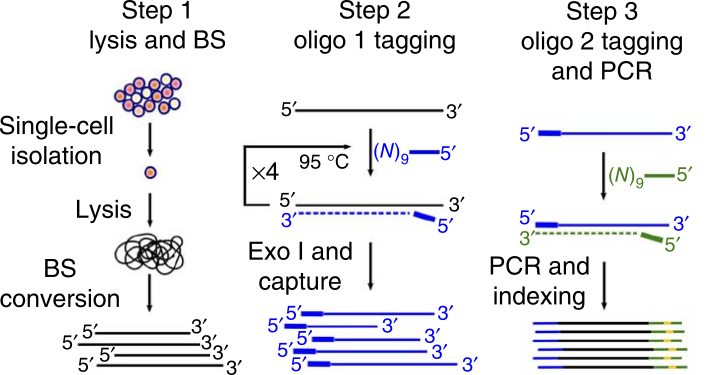
\includegraphics[width=10cm]{./ims/smallwood2014.png}
%\caption[\acrshort{scbs-seq} workflow]{\textbf{\acrshort{scbs-seq} workflow.} Single cells are collected by \acrshort{facs} and lysed separately. After bisulfite treatment, the 5' sequencing adapter is added by random priming and extension. The 3' sequencing adapter is added by the same mechanism, and the library is amplified, indexed and sequenced. Taken from \cite{smallwood2014}.}
%\label{fig:smallwood2014}
%\end{figure}
%
%\citeauthor{smallwood2014} applied \acrshort{scbs-seq} to 12 metaphase II oocytes and 20 mouse \acrfullpl{esc}. On average, only 17.7\% of known \acrshort{cpg} sites could be recovered at a sequencing depth of 3.9 million mapped reads per cell. Due to sensitivity limitations, \citeauthor{smallwood2014} suggest that \acrshort{scbs-seq} may be used to generate bulk methylation profiles from small samples of rare cells. Despite the low sensitivity achieved, the authors were able to identify \acrshort{5mc} heterogeneity in \acrshortpl{esc}. \citeauthor{smallwood2014} also propose that finding a way to amplify methylated genomic \acrshort{dna} before bisulphite conversion could help recover more \acrshortpl{cpg}. \acrshort{scbs-seq} can thus far not distinguish between \acrshort{5mc} and 5-hydroxymethylcytosine, which has recently been shown to be an intermediate product in \acrshort{dna} demethylation \citep{wu2017}.\pms

\subsection{Microwell scATAC-seq}
\label{subsect:lit_microwell_scatac-seq}
% The principles and significance of bulk \acrshort{atac-seq} have already been explained in section \ref{subsect:lit_atac-seq}. Single-cell chromatin accessibility data can help us understand differences in gene regulation between cells. So far, a number of single-cell \acrshort{atac-seq} (\acrshort{scatac-seq}) methods have been developed \citep{buenrostro2015, cusanovich2015, mezger2018}. As these methods employ microfluidic cell loading or combinatorial indexing, they will be explained in sections \ref{sec:lit_microarrays} and \ref{sec:lit_splitting_pooling} respectively.\pms

% \todo[inline]{more details on atac-seq data please. \cite{mezger2018} use expensive robot}

A \acrshort{scatac-seq} approach which does not explicitly require the use of microfluidics was published in \citeyear{chen2018} by the Teichmann Group \citep{chen2018}. Their protocol relies on an interesting peculiarity about Tn5: when Tn5 binds to accessible chromatin, it cleaves chromosomal \acrshort{dna} and inserts its adapters at the 5' end of each opposite strand. However, during this process, Tn5 remains clamped on the \acrshort{dna} strand until it is denatured by either \acrshort{sds} or a heat shock \citep{picelli2014b}. During this process, the cell is lysed, but its \acrshort{dna} content stays confined to the nucleus. Only upon denaturation of Tn5, the fragmented \acrshort{dna} is released from the enzyme. In the Teichmann protocol, bulk tagmented nuclei are sorted into a microtiter plate containing lysis buffer. The tagmentation reaction is then stopped using \acrshort{sds} and further reactions are performed separately in each microwell. An overview of the technique is shown in figure \ref{fig:chen2018_edited}.\pms

\begin{figure}[ht]
	\centerfloat
	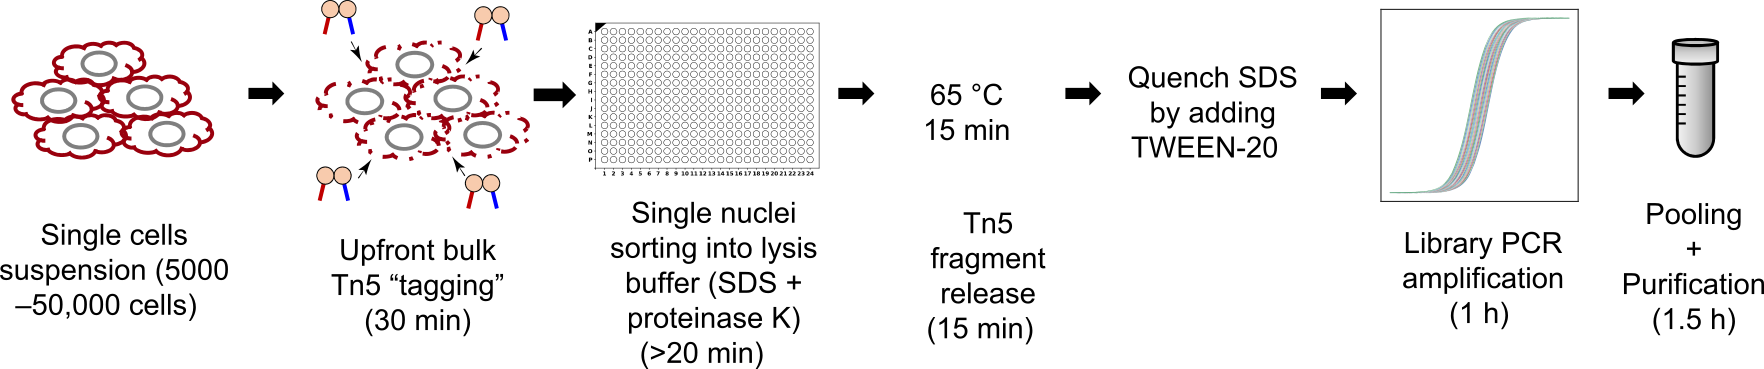
\includegraphics[width=\textwidth]{./ims/chen2018_edited.png}
	\caption[Teichmann \acrshort{scatac-seq} workflow]{\textbf{Teichmann \acrshort{scatac-seq} workflow.} Tagmentation is performed in bulk by incubating 50 000 cells with Tn5 transposase. "Tagmented" nuclei are sorted into 384-well plates containing lysis buffer with \acrshort{sds} and proteinase K, which inactivate Tn5. After Tn5 is inactivated and \acrshort{dna} fragments are released, \acrshort{sds} is quenched by addition of Tween-20, preventing non-specific inactivation of downstream enzymes. Fragments generated by Tn5 are then indexed using indexing \acrshort{pcr}, amplified, pooled and sequenced. Taken from \cite{chen2018}.}
	\label{fig:chen2018_edited}
\end{figure}

In contrast to earlier \acrshort{scatac-seq} protocols, the Teichmann protocol does not require intermediate purification of the \acrshort{dna}, simplifying the tagmentation workflow. \citeauthor{chen2018} benchmarked their \acrshort{scatac-seq} method against the \citeauthor{buenrostro2015} C1 \acrshort{scatac-seq} protocol (which will be shown in section \ref{sec:lit_microarrays}) and found that their own protocol generated higher quality data in a shorter time frame. The whole procedure takes place in the same plate and does not require intermediate purification steps, as opposed to previous \acrshort{scatac-seq} protocols which employ bead purification of \acrshort{dna} after tagmentation. \citeauthor{chen2018} also show that immunostained cells retain their staining after bulk tagmentation, meaning \acrshort{facs} can be used to filter rare cell types from the sample post-tagmentation. Additionally, the bulk tagmentation approach cuts cost of Tn5 per cell considerably but the subsequent microcompartment-based approach still incurs a substantial cost due to the \SI{20}{\micro\litre} \acrshort{pcr} reaction volume.\pms

% \todo[inline]{let's keep the details for later, but apparently the C1 protocol takes an additional 4 hours as well}

\newpage
\subsection{Microwell Approaches: Key Takeaway}
Due to their user-friendliness and modest requirements in terms of equipment, the use of plate-based techniques has become widespread. However, microcompartment-based single-cell analysis techniques suffer from a number of inherent disadvantages:

\begin{enumerate}
	\setlength{\itemsep}{0pt}%
	\setlength{\parskip}{0pt}%
	\item Isolating and/or sorting single cells into microwells and performing reactions on them is tedious, especially when performed manually. \acrshort{facs} and automated liquid handling may be used to partially solve these problems.
	\item Performing single-cell reactions in a microwell plate leads to large reagent volumes per cell, resulting in a high cost and, more importantly, decreased reaction efficiency due to dilution effects \citep{wu2014}.
	\item Handling reaction plates can form a throughput bottle neck in parallel processing of a large number of cells, for example during reverse transcription, where one heat block can only process 96 cells.
	% 96 cells require a full 96-well plate, whereas if each cell is confined in a droplet potentially thousands of cells could be handled in a single well.
\end{enumerate}

Despite these drawbacks, microcompartment-based techniques have proven to be viable tools to extract information on single-cell resolution \acrshort{dna} methylation, chromatin condensation, gene expression and genomic profile. Generally speaking, microcompartment techniques such as \acrshort{smart-seq} and \acrshort{cel-seq} yield data of higher quality than the high-throughput methods shown later \citep{ziegenhain2017}. Together, the protocols explained in this sections have led to a number of groundbreaking results of which a limited selection will be shown in \ref{sec:lit_applications}.\pms

The greatest advantage that microwells offer can be found not in accuracy, cost or throughput, but in flexibility. It is straightforward to manipulate and sample the contents of a microwell plate to optimise the reactions carried out within. Moreover, multi-step methods involving sequential addition and purification can easily be carried out on an accessible well platform. Many high-throughput techniques shown in the following sections were born in a microwell, and most likely some of the more complicated techniques we will see in the future will start in a well as well.\pms

\newpage
\section{Microfluidic Arrays}
\label{sec:lit_microarrays}
The previous section has shown how single-cell data can be obtained by simply applying bulk analysis methods to a single cell in a microwell. A major bottleneck in the application of these assays is the distribution of single cells into individual microcompartments. Common methods include manual picking, \acrshort{facs} or Poisson-distributed dilution, each with their own set of disadvantages. In the following section, a number of techniques which separate or trap single cells into (sub)nanolitre volume compartments are introduced.\pms

\subsection{Fluidigm C1}
\label{subsect:lit_fluidigm_c1}
% The Fluidigm C1 was first presented by Stephen Quake and colleagues at the MicroTAS 2014 conference as a single cell isolation platform for whole genome sequencing.
The C1 comprises a benchtop microfluidic controller that contains the pneumatic hardware, and a disposable \acrfull{ifc} (figure \ref{fig:c1}), which hosts the microfluidic channels through which the sample is routed. Together, they form a platform that can isolate single cells from dilute cell suspensions into nanolitre capture sites. In section \ref{sec:lit_well-based}, we briefly mentioned that the \acrshort{smart-seq}2 protocol can be implemented on the C1. Preceding \acrshort{smart-seq}2, \citeauthor{buenrostro2015} published a C1-based \acrshort{scatac-seq} protocol \citep{buenrostro2015}. Here, tagmentation and \acrshort{pcr} occur on the C1 \acrshort{ifc}, after which single-cell libraries are collected and further amplified with cell-identifying barcoded primers. For an overview of the \citeauthor{buenrostro2015} scATAC-seq method, see figure \ref{fig:buenrostro2015}.\pms

%\todo[inline]{mention some statistics here, also mention scrna-seq and show gene numbers etc}\pms

\begin{figure}[ht]
	\centerfloat
	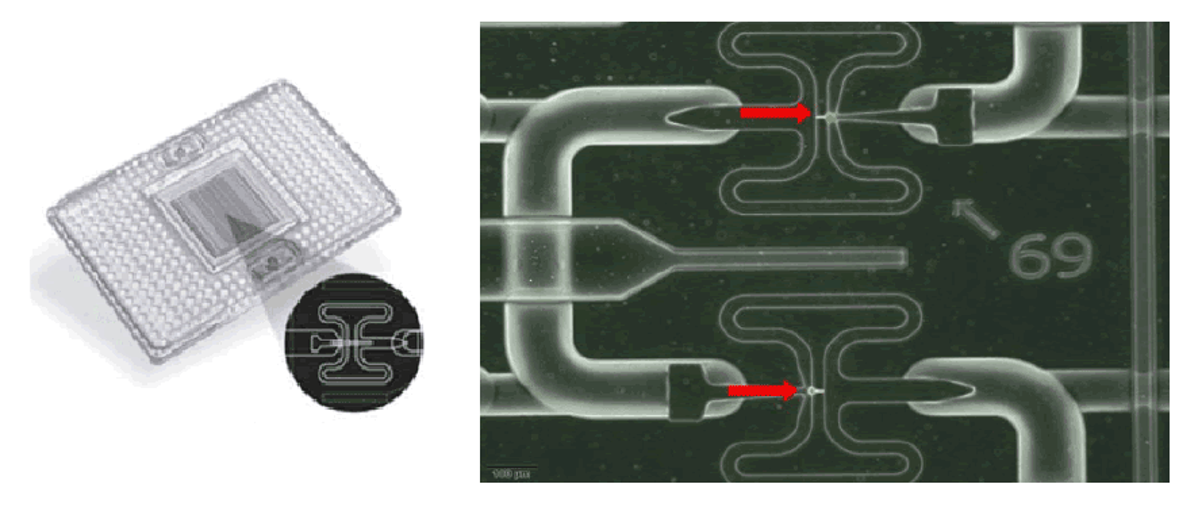
\includegraphics[width=12cm]{./ims/c1.png}
	\caption[Fluidigm C1 \acrshort{ifc}]{\textbf{Fluidigm C1 \acrshort{ifc}.} A suspension of single cells is added to the \acrshort{ifc}'s sample inlet and inserted into the C1 control unit. The control unit pneumatically pumps the suspension through a serpentine channel containing a series of capture sites. Once a cell occupies a capture site, access to the site's collection chamber is blocked, routing subsequent cells to the next capture site. This results in a series of capture sites along the path each containing a single cell. After a run time of 1 hour, cell occupancy is checked using (fluorescence) microscopy. Then, lysis reagents are routed through the serpentine channels, lysing cells and clearing the obstructed path to the collection chambers, resulting in a flow of lysate from each capture site to its respective collection chamber. Next, reverse transcription or amplification reagents can be routed to the chamber. The reaction products from individual cells are then collected into a separate microwell. During each microfluidic unit operation, a set of peristaltic valves seal off every capture site in order to minimise contamination. Adapted from \cite{azizi2014}.}
	\label{fig:c1}
\end{figure}

\begin{figure}[ht]
	\centerfloat
	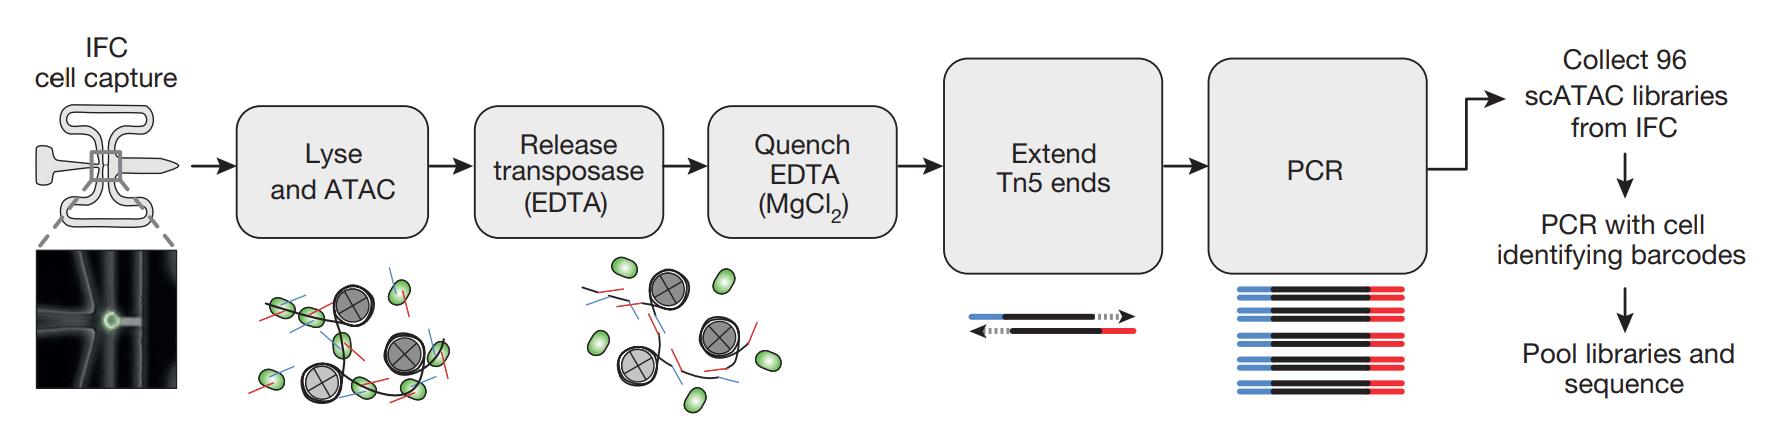
\includegraphics[width=\textwidth]{./ims/buenrostro2015.png}
	\caption[Buenrostro \acrshort{scatac-seq}]{\textbf{Buenrostro \acrshort{scatac-seq}.} \SI{5}{\micro\litre} of a 300 cells/\SI{}{\micro\litre} suspension is placed into the \acrshort{ifc} sample inlet. Single cells are trapped into capture sites and lysed. In an individual reaction chamber, each cell is tagmented in \SI{13.5}{\nano\litre} of tagmentation mix. After \acrshort{edta}-mediated release of Tn5, the tagged fragments are pre-amplified by \acrshort{pcr} on-chip. After amplification, individual cell samples are collected and individually barcoded using \acrshort{pcr}. Only then are the single-cell libraries collected and pooled for sequencing. Taken from \cite{buenrostro2015}.}
	\label{fig:buenrostro2015}
\end{figure}

The greatest advantage of the C1 compared to conventional microwells are ease of use and semi-automation at a minimal loss of data quality. During cell trapping, tagmentation and pre-amplification, minimal human interference is necessary. However, barcoding and subsequent amplification of the single-cell libraries still need to happen in a microwell plate. The C1 approach is therefore practically an automated cell-capture and nucleic acid capture method followed by microcompartment-style barcoding. As the \acrshort{ifc} can only process 96 cells in parallel, high-throughput application of the C1 is difficult. Moreover, the C1 \acrshort{ifc} only accommodates three cell size classes per chip design (5-10, 10-17 and 17-25 \SI{}{\um} in diameter), leading to a size-biased selection. The very nature of the C1's cell trapping mechanism also complicates the capture of non-spherical cells. \citeauthor{macosko2015}, authors of a competing microfluidic \acrshort{scrna-seq} method covered in section \ref{subsect:lit_drop-seq}, report that 30\% of C1-generated libraries contain mixed-species contamination, which is unusually high for single-cell methods \citep{macosko2015}. \citeauthor{shalek2014} report a more forgiving multiplet rate of 11\%. Additionally, the 96-cell \acrshort{ifc} takes an input sample of at least 1000 cells, imposing an effective capture efficiency of 1-10\% \citep{zilionis2017}. This last drawback prohibits the application of C1-based cell capture on protocols where information on rare cell types is key, such as de novo cell typing. It is due to these limitations and strong competition from droplet microfluidics approaches that the C1 has not been able hold a large market share, appearing in 228 publications over a span of 8 years \citep{fluidigmwebsite2019}, compared to 391 publications for the 10x Chromium, which was released in 2016. Still, the C1 has found niche applications in the automisation of specialised and complicated protocols such as \acrshort{sci-car} (see section \ref{sec:lit_splitting_pooling}).\pms

% \todo[inline]{put something here about custom protocols on the C1, compare to number of 10x publications in 2 years. Price? when it came out, 23 dollars per cell. add some stuff about cool new protocols on the C1, the machine is not dead yet}

\subsection{Seq-Well}
\label{subsect:lit_seq-well}
A rather straightforward microfluidic cell loading strategy dubbed Seq-Well was published in \citeyear{gierahn2017} \citep{gierahn2017}. In this method, cells and beads carrying barcoded poly-dT primers are loaded into an array of picolitre wells. Here, the barcoded poly-dT primers capture cellular \acrshort{mrna}. The beads are then pooled for bulk reverse transcription. An overview of the Seq-Well method is given in figure \ref{fig:gierahn2017}.\pms

\begin{figure}[ht]
	\centerfloat
	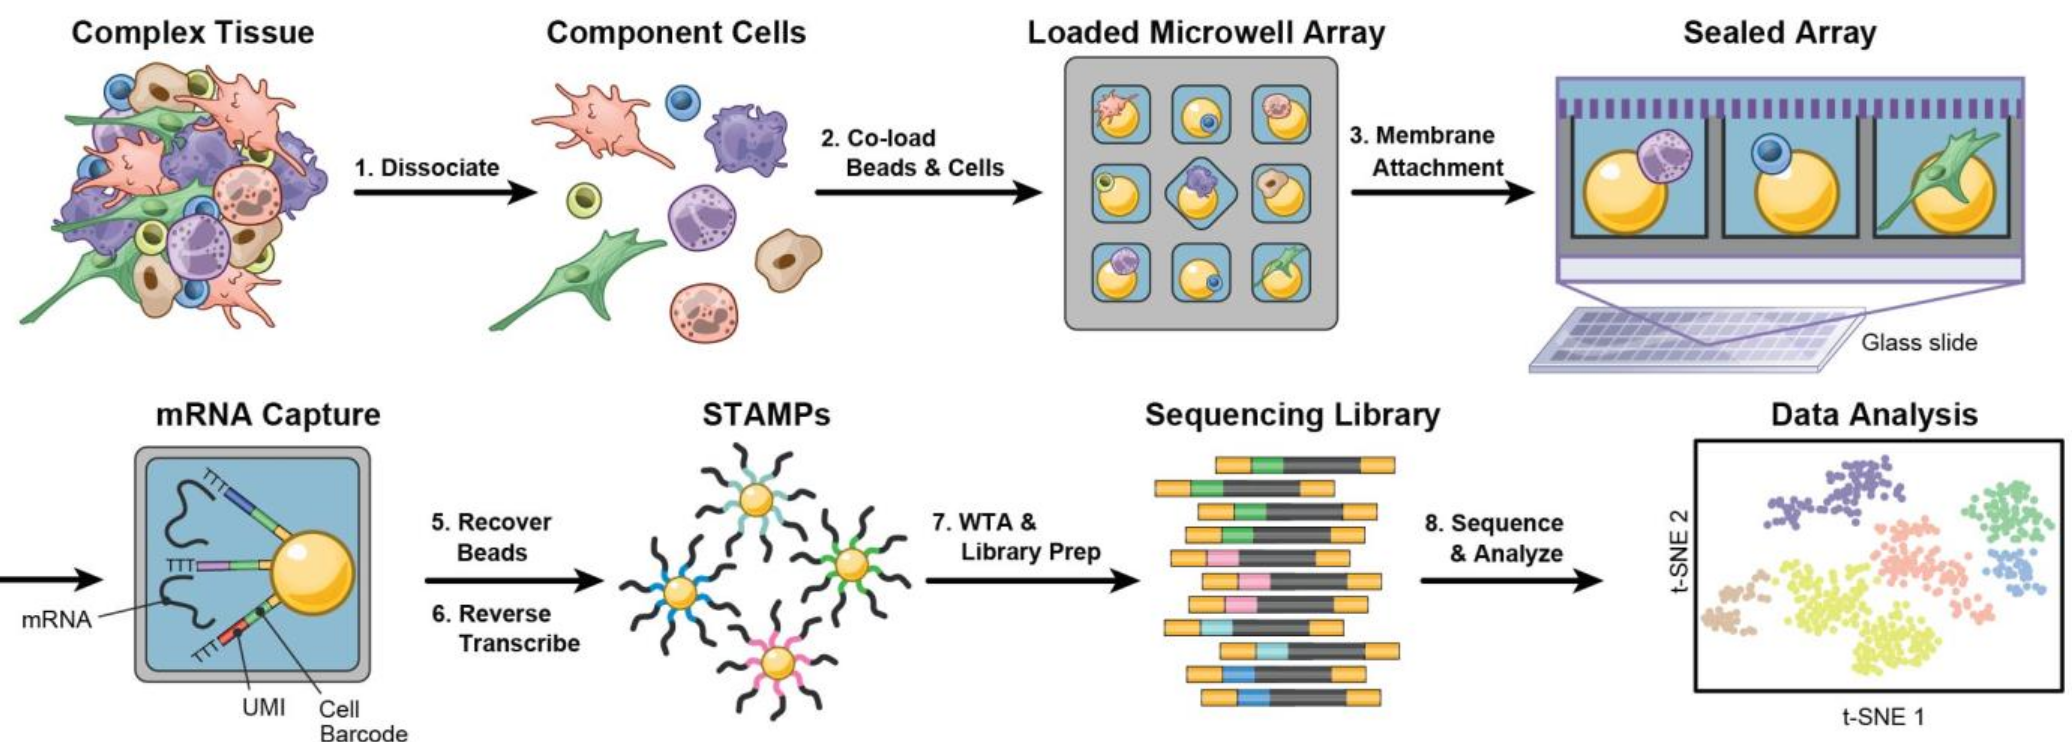
\includegraphics[width=\textwidth]{./ims/gierahn2017.png}
	\caption[Seq-Well cell loading and library generation]{\textbf{Seq-Well cell loading and library generation.} Cells are co-loaded together with barcoded microbeads in a \acrshort{pdms} array containing 83 200 picowells. Each bead oligo holds a cellular barcode, a \acrshort{umi} and a poly-dT tail to capture \acrshort{mrna} poly-A tails. The wells are then sealed using a semi-permeable membrane and submerged in lysis buffer. In each well, released cellular \acrshort{mrna} is captured by the poly-dT primers on the barcoded beads. The plates are unsealed, and beads are pooled. A bulk template-switching reverse transcription reaction then generates the \acrfullpl{stamp}, which are then amplified and sequenced. Adapted from \cite{gierahn2017}.}
	\label{fig:gierahn2017}
\end{figure}

Seq-Well improves on earlier picowell methods by \cite{fan2015} and \cite{yuan2016} by chemically sealing the array of picolitre wells using semi-permeable membrane which allows for buffer exchange, but prevents cross-contamination between wells. The inner surface of the picowells is also treated to prevent non-specific \acrshort{mrna} binding. Similarly to \acrshort{smart-seq}, Seq-Well uses a template-switching library generation strategy to facilitate amplification and to produce full-length transcripts. In short, Seq-Well is a simple and portable protocol for loading a large number of cells into microwells rapidly. However, \citeauthor{zilionis2017} remark that not all \acrshort{mrna} is capture by the barcoded beads, possibly leading to contamination at the pooling step after hybridisation \citep{zilionis2017}. \citeauthor{gierahn2017} also observed a multiplet rate of 11.4\% when 20 000 of the 83 200 available picowells were loaded with cells. 77.5\% of the Seq-Well reads could be mapped to a reference exome and {\textasciitilde}6 000 human genes were detected. This is higher than droplet-microfluidics techniques such as Drop-seq ({\textasciitilde}5 000 human genes) and 10x Chromium ({\textasciitilde}4 600 human genes) but lower than a true microwell protocol such as \acrshort{smart-seq}2 ({\textasciitilde}12 000 human genes).\pms

\subsection{Microfluidic Arrays: Key Takeaway}
Microfluidic array methods have succeeded in reducing the significant labour costs associated with single-cell experiments. As always, a trade-off is made between data complexity and throughput. Single-cell experiments on the Fluidigm C1 platform offer high quality data consistent with explicit well-based techniques, but at a high cost and low throughput while Seq-Well offers high-throughput, portability and low cost at the expense of sensitivity and specificity. Importantly, both methods still allow customisation and adaptation of the reactions performed on the isolated cells. Microfluidic array techniques therefore form an intermediate between well-based protocols and the droplet-microfluidic techniques shown in section \ref{sec:lit_dropletmicrofluidics}.\pms

\newpage
\section{Droplet Microfluidic Single Cell Omics Techniques}
\label{sec:lit_dropletmicrofluidics}
 In \citeyear{klein2015}, two remarkable \acrlong{scrna-seq} methods debuted in the same issue of Cell \citep{klein2015, macosko2015}. Two research groups both affiliated with Harvard university had collaboratively come up with the idea of barcoding cells by encapsulating them together with solid primer carriers in microscopic droplets. The methods, aptly named inDrop and Drop-seq, both relied on encapsulating single cells in tiny water-in-oil droplets together with a microbead carrying the barcoded primers used to index every cell's \acrshort{mrna} content. The following section will briefly cover inDrop and Drop-seq and, as the experimental section of this thesis revolves around a hybrid version between the two, their differences will be examined closely.\pms

\newpage
\subsection{Drop-seq}
\label{subsect:lit_drop-seq}
Drop-seq, \citeauthor{macosko2015}'s approach to droplet-based \acrlong{scrna-seq}, is based around co-encapsulating single cells with a barcoded resin bead on a microfluidic chip. Inside every droplet, the cell's \acrshort{mrna} content is captured by the bead's barcoded transcription primers. The ensuing reverse transcription reaction incorporates the primer's barcode and \acrfull{umi} in the \acrshort{cdna}, which allows researchers to demultiplex the \acrshort{cdna} by cell and \acrshort{mrna} transcript of origin. Drop-seq's bead production process, microfluidic chip and workflow are given in figures \ref{fig:macosko2015_1}-\ref{fig:macosko2015_3}.\pms

\begin{figure}[ht]
	\centerfloat
	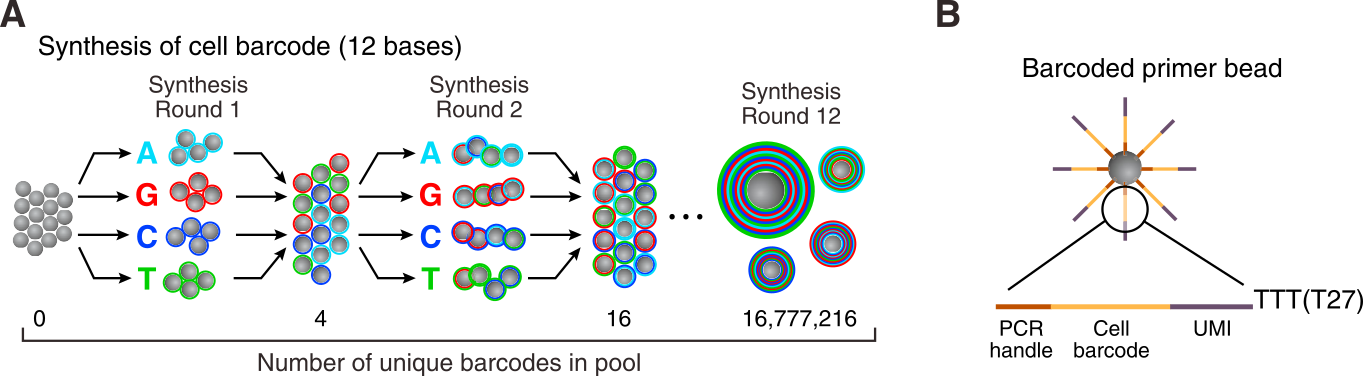
\includegraphics[width=\textwidth]{./ims/macosko2015_1.png}
	\caption[Drop-seq barcoded bead generation]{\textbf{Drop-seq barcoded bead generation.} (A) Resin beads undergo successive rounds of splitting, oligo synthesis and pooling to generate 2\textsuperscript{12} = 16 777 216 possible uniquely barcoded beads. Then, eight steps of degenerate synthesis append an eight nucleotide \acrshort{umi} to the cell barcodes, followed by addition of a poly-T tail which can capture cellular \acrshort{mrna}. (B) Overview of the final bead barcode structure. Taken from \cite{macosko2015}.}
	\label{fig:macosko2015_1}
\end{figure}

\begin{figure}[ht]
\begin{minipage}[]{0.5\textwidth}
	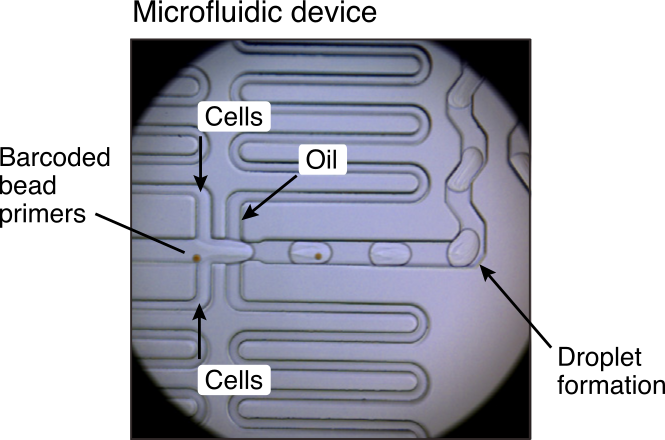
\includegraphics[width=\textwidth]{./ims/macosko2015_2.png}
\end{minipage}\hfill
\begin{minipage}[]{0.45\textwidth}
	\captionsetup{margin={0pt,18pt}, labelfont=bf}
	\caption[Drop-seq microfluidic chip]{\textbf{Drop-seq microfluidic chip.} A flow of barcoded beads suspended in lysis buffer is joined by a single-cell suspension and emulsified into nanolitre droplets by an oil flow. Taken from \cite{macosko2015}.}
	\label{fig:macosko2015_2}
\end{minipage}
\end{figure}

\begin{figure}[ht]
	\centerfloat
	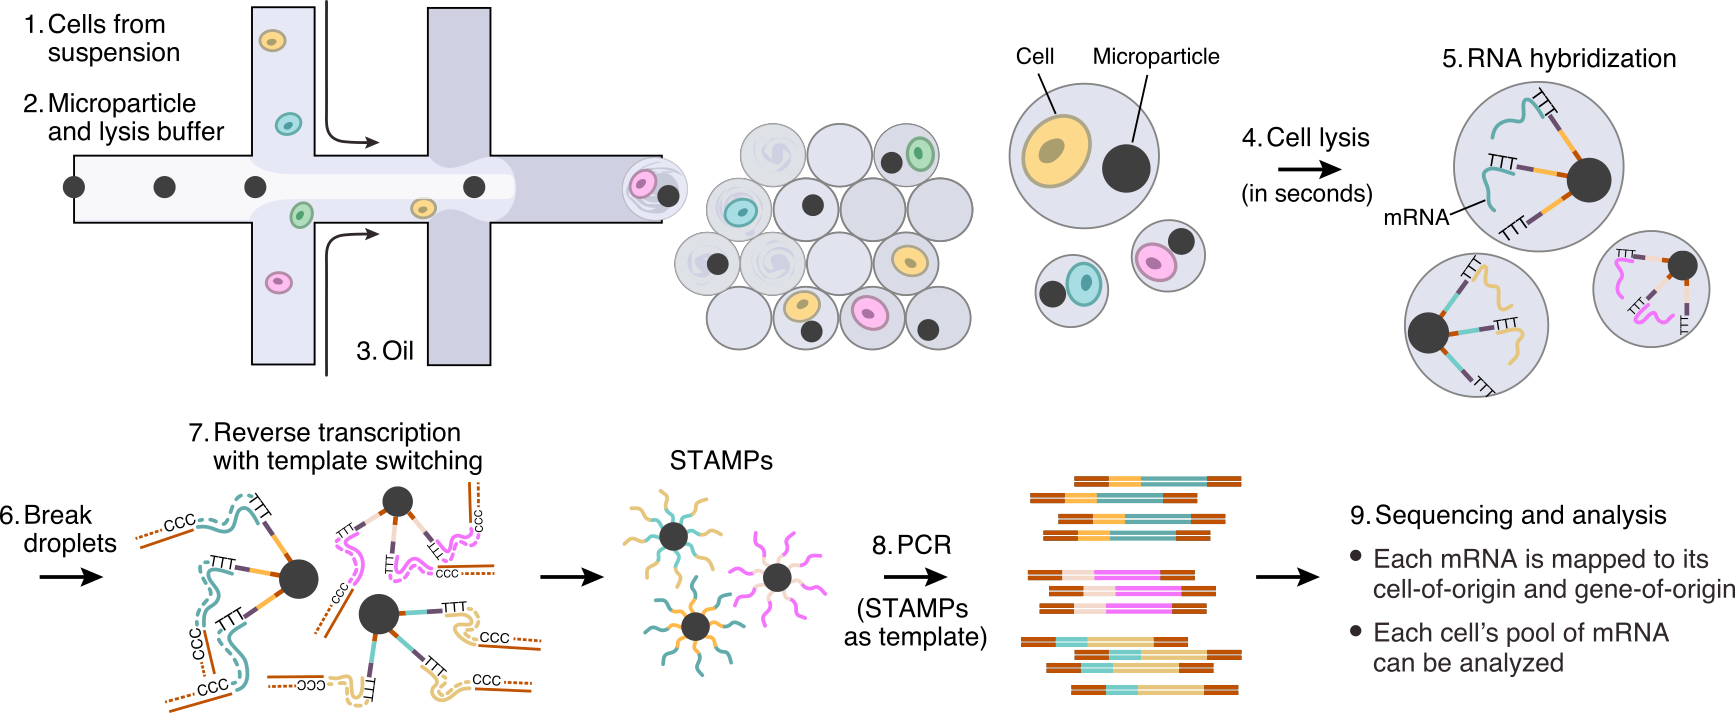
\includegraphics[width=\textwidth]{./ims/macosko2015_3.png}
	\caption[Drop-seq library generation]{\textbf{Drop-seq library generation.} Single cells are encapsulated in a nanolitre volume droplet together with a barcoded resin bead and lysis buffer. The surface of each bead is covered in millions of copies of a bead-specific barcoded poly-dT primer which captures \acrshort{mrna} released by the cells in the droplets. The beads are then pooled in a large volume of water, which prevents further hybridisation outside of the droplet. Immediately after, the hybridised \acrshort{mrna} libraries are copied to the bead primers by template-switching reverse transcription, generating a library of \acrfullpl{stamp}. The \acrshort{stamp} libraries are \acrshort{ispcr}-amplified, fragmented, \acrshort{pcr}-amplified again and sequenced. The last \acrshort{pcr} preferentially amplifies 3' fragments, leading to a 3'-enriched sequencing library. After sequencing, the cellular barcode is used to identify each transcript's cell of origin, and the \acrshort{umi} is used to count individual transcripts. Taken from \cite{macosko2015}.}
	\label{fig:macosko2015_3}
\end{figure}

Using Drop-seq, a single researcher can prepare thousands of single cell transcriptomes for sequencing in a single day, orders of magnitude faster than the 96-well plate assays discussed in section \ref{sec:lit_well-based}. In the original Drop-seq paper, \citeauthor{macosko2015} profiled 44 808 single-cell mouse retina transcriptomes in just 4 days, at a fraction of the cost of conventional microwell-based due to the ultra low reaction volumes (\textasciitilde{}\SI{1}{\nano\litre}). Whereas the price of \acrshort{smart-seq} is estimated at \$3 - \$30 per cell before sequencing, a Drop-seq run indexes single cells at \$0.1 - \$0.65 per cell \citep{macosko2015, ziegenhain2017}. Drop-seq's incredible throughput potential is paired with a number of important drawbacks, a major one being reduced \acrshort{mrna} capture efficiency and sensitivity compared to well-based protocols. Using spiked-in \acrshort{rna} standards, \citeauthor{macosko2015} estimate that Drop-seq captures \textasciitilde{}12\% of the cellular \acrshort{mrna} and can detect an average of 44 295 \acrshort{mrna} transcripts from 6 722 genes in \acrshort{hek} cells. This is significantly lower than \acrshort{smart-seq}2, which captures \textasciitilde{}20\% of cellular \acrshort{mrna} and detects 12k genes in the same cell line \citep{picelli2013}. It is important to note that both Drop-seq and \acrshort{smart-seq} use the same path of template-switching \acrshort{rt} followed by \acrshort{ispcr} and subsequent Illumina Nextera XT sequencing library preparation. However, Drop-seq selectively \acrshort{pcr}-amplifies 3' fragments since this is where the cellular barcode is located. Other fragments can simply not be assigned to a cell of origin and are therefore suppressed in the final sequencing library. This means that Drop-seq can absolutely quantify transcripts by mapping the 3' ends to a reference exome, but cannot give information on distal transcript regions.\pms

Another important limitation of Drop-seq is low cell capture efficiency. Since co-encapsulation of two independent particles is a double-Poissonian process, both cell and bead concentrations need to be kept low in order to minimise multiplet encapsulation. At the concentrations used by \citeauthor{macosko2015}, the chance for a droplet to receive either a bead or a droplet is \textasciitilde{}1-5\%. This leads to a dual occupancy rate of only \textasciitilde{}0.1\% and an effective cell capture efficiency of just \textasciitilde{}5\% of the input sample. \citeauthor{macosko2015} suggest that Drop-seq's low capture efficiency can be compensated by simply brute-force processing a large number of cells. This is shown in the original publication, where rare cells constituting 0.1\%-0.9\% of the population are successfully characterised when thousands of cells are analysed.\pms

\subsection{inDrop}
\label{subsect:lit_indrop}
Published concurrently with Drop-seq, inDrop ("\textit{ind}exing \textit{drop}lets") is a different approach to the same concept. Again, single cells are encapsulated in nanolitre droplets together with reverse transcription reagents and beads carrying barcoded poly-dT primers \citep{klein2015, zilionis2017}. The inDrop bead production process, microfluidic chip and workflow are shown in figures \ref{fig:klein2015_1}-\ref{fig:klein2015_3}.\pms

\begin{figure}[ht]
	\centerfloat
	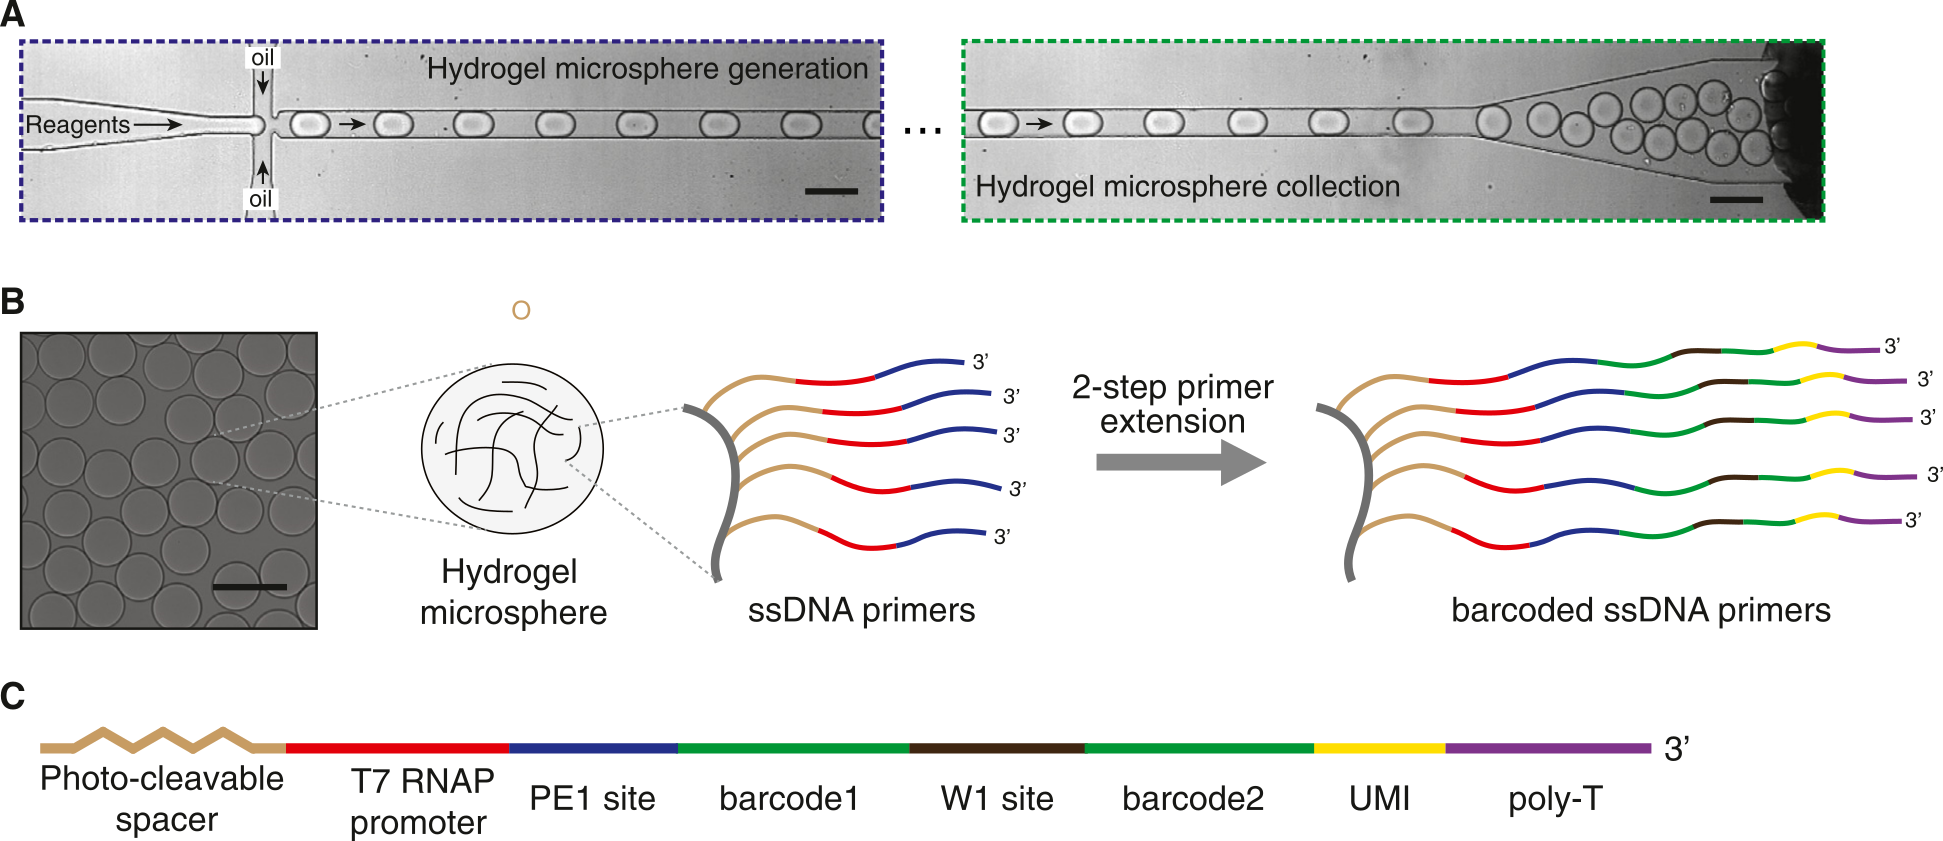
\includegraphics[width=\textwidth]{./ims/klein2015_1.png}
	\caption[inDrop barcoded bead generation]{\textbf{inDrop barcoded bead generation.} (A) Millions of polyacrylamide microspheres are produced by droplet microfluidics and polymerised to hydrogel beads. (B) Short \acrshort{dna} primers in the acrylamide matrix serve as a \acrshort{pcr} priming site and allow a photocleavable spacer, T7 \acrshort{rna} promoter to be appended. After two successive steps of splitting and pooling \acrshort{pcr} in 384 wells, each hydrogel carries one of 147 456 (= 384 x 384) possible cellular barcodes. (C) The hydrogel primers also carry a \acrshort{umi} and a poly-T tail. Taken from \cite{klein2015}.}
	\label{fig:klein2015_1}
\end{figure}

\begin{figure}[ht]
	\centerfloat
	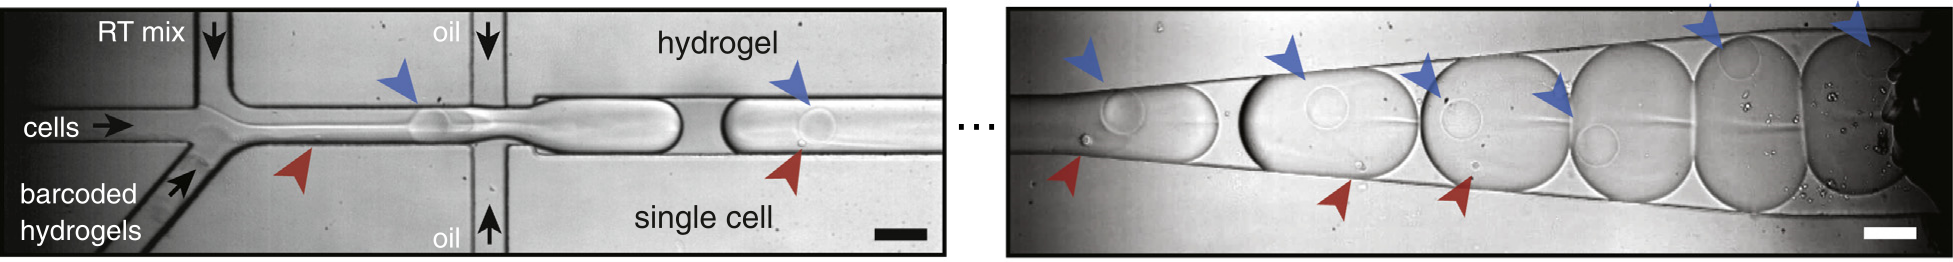
\includegraphics[width=\textwidth]{./ims/klein2015_2.png}
	\caption[inDrop microfluidic chip]{\textbf{inDrop microfluidic chip.} A dilute cell suspension is joined by a flow of reverse transcription reagents and stacked hydrogels, and further emulsified by flow-focusing. Taken from \cite{klein2015}.}
	\label{fig:klein2015_2}
\end{figure}

\begin{figure}[ht]
	\centerfloat
	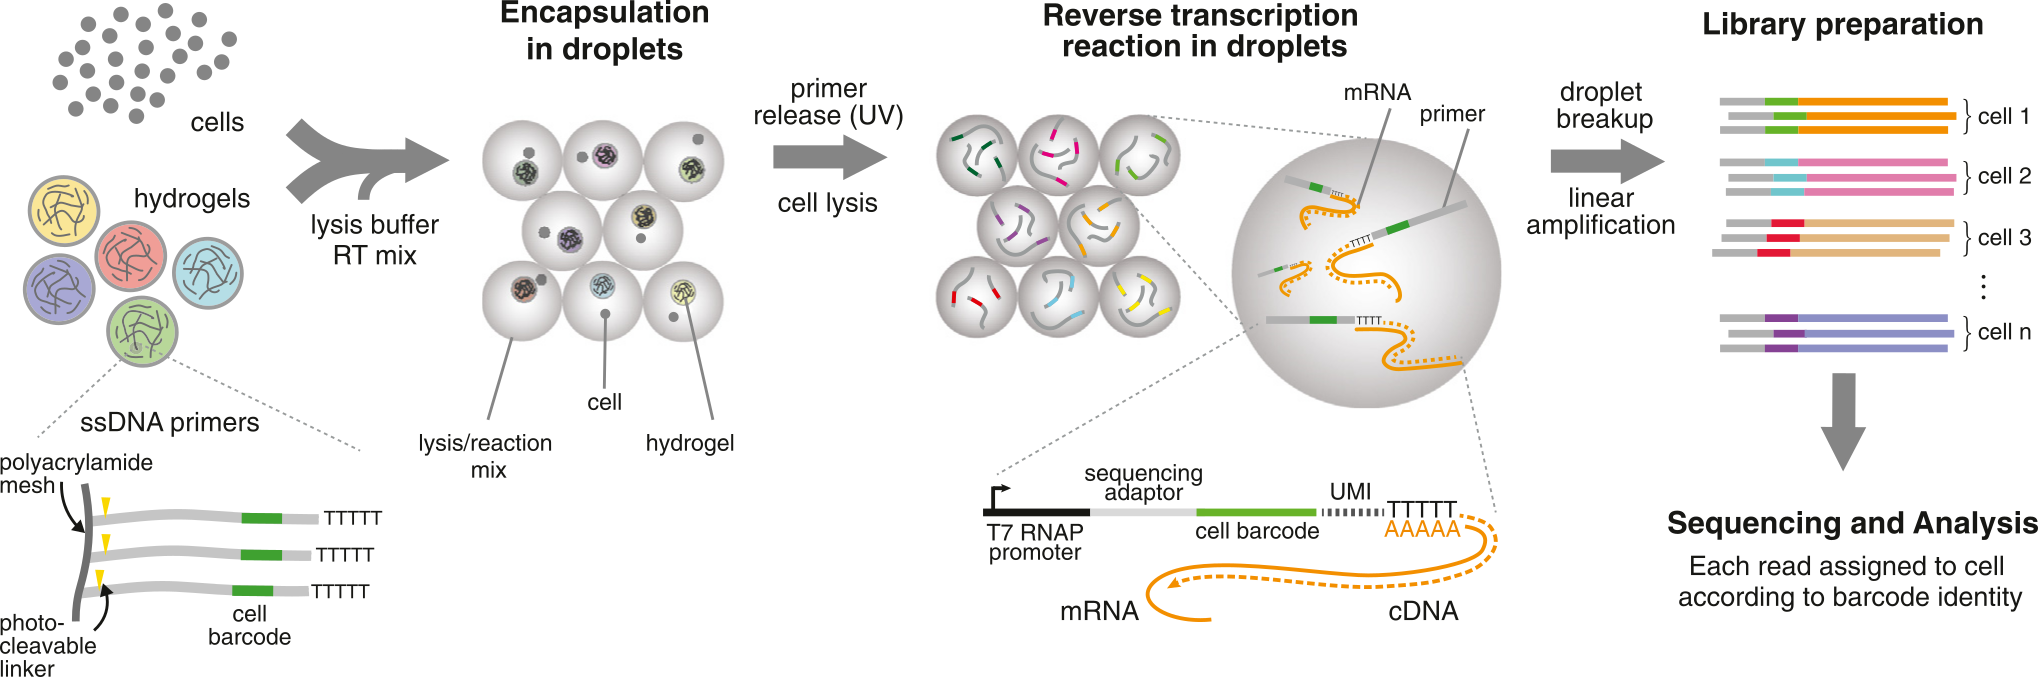
\includegraphics[width=\textwidth]{./ims/klein2015_3.png}
	\caption[inDrop library generation]{\textbf{inDrop library generation.} Similarly to Drop-seq, single cells are encapsulated in a nanolitre volume droplet together with a barcoded hydrogel bead. Each hydrogel bead carries a payload of bead-specific barcoded poly-dT primers covalently incorporated in the gel matrix. These primers are released from the hydrogel using a \acrshort{uv}-cleavable chemical linker. The cell is lysed and its \acrshort{mrna} content is reverse transcribed with the released hydrogel primers in the droplet. The resulting barcoded \acrshort{cdna} fragments are pooled and linearly amplified using \acrshort{ivt}, similar to \acrshort{cel-seq}. After sequencing, each transcript's cellular barcode and \acrshort{umi} are used to identify cell and transcript of origin. Taken from \cite{klein2015}.}
	\label{fig:klein2015_3}
\end{figure}

Though both methods share a central concept, several important differences distinguish inDrop from Drop-seq. One of the most important differences can be found in the nature of the primer-loaded beads - whereas Drop-seq uses hard, \SI{30}{\micro\metre} plastic beads, inDrop uses \SI{70}{\micro\metre} soft, deformable hydrogels. These hydrogels are loaded into the microfluidic chip at concentrations \textasciitilde{}100 times higher than Drop-seq's beads, allowing them to stack inside the chip's microfluidic channels. Near the end of the funnel, a single, lined-up file of beads is formed and pushed towards the cell flow. As the release of beads can be controlled directly, flows can now be tuned so that nearly 100\% of droplets contain at least one bead \citep{klein2015, abate2009}. Due to this "super-Poissonian" stochastic bead loading, inDrop attains a cell-capture rate of near 95\%, compared to Drop-seq's 5\%. This allows inDrop to be applied to scenarios where the sample does \textit{not} permit brute-force analysis of thousands of cells, for example in a clinical context.\pms

Another important difference between Drop-seq and inDrop is the post-encapsulation library preparation. Whereas Drop-seq is strongly \acrshort{smart-seq} inspired, inDrop essentially follows the \acrshort{cel-seq}/\acrshort{mars-seq} (a high-throughput implementation of \acrshort{cel-seq}) library preparation process \citep{hashimshony2012, jaitin2014}. Like \acrshort{cel-seq}, the inDrop \acrshort{cdna} libraries are pooled, in-vitro transcribed for linear amplification and fragmented/\acrshort{pcr} enriched for sequencing. Due to this overnight in-vitro transcription step, inDrop has a higher fixed time cost than Drop-seq. Using \acrshort{ercc} spike-ins, \citeauthor{klein2015} estimate inDrop's \acrshort{mrna} capture efficiency at 7.1\% - higher than \acrshort{cel-seq}'s 3.4\%, but lower than \acrshort{smart-seq}2 and \acrshort{cel-seq}2's \textasciitilde{}20\% \citep{klein2015, grun2014, picelli2013, hashimshony2016}. inDrop is thus plagued by the same low sensitivity issues as Drop-seq.\pms

% \subsection{10x Chromium}
%\label{subsect:lit_10x_chromium}
% The Chromium is an inDrop-like microfluidic single-cell platform released by 10x Genomics in 2016. It
% -> not elastomer (list advantages of hard cartridge), works very well and easy to use BUT costly

\subsection{Droplet Microfluidic Techniques: Key Takeaway}
As shown above, droplet-microfluidic single-cell techniques offer several advantages, most notably throughput. A single researcher can now process 10 000 single cells for sequencing in 12 hours, at a fraction of the cost of microwell-based assays. As the actual cell encapsulation step takes only minutes, throughput can be increased further by simply encapsulating more cells and processing their emulsions together. The ultra-low reaction volumes (\SI{}{\nano\litre}) associated with microfluidics strongly reduce cost, which can be further minimised when cell/bead dual occupancy are optimised. Moreover, these low reactions volumes have been shown to reduce technical noise and increase product yield \citep{streets2014}. However, despite this supposed increase in reaction efficiency, all droplet microfluidic single-cell techniques exhibit significantly lower sensitivity when compared to their microwell counterparts. Two considerations need to be made regarding this observation. First, sequencing depth, a deciding factor in the data quality of single-cell experiments, is usually much lower in high-throughput methods due to the high number of cells processed per sample. It is often difficult or prohibitively costly to sequence thousands of single-cell transcriptomes from the same tissue sample to saturation. Hopefully, the ongoing decrease of \acrshort{ngs} price will mitigate this limitation in the future. Second, Drop-seq and inDrop are often compared with newer generation of microwell methods such as \acrshort{smart-seq}2 and \acrshort{cel-seq}2. Over the years, these methods have been heavily optimised in terms of reagent concentrations, enzymes, incubation times and so on. Several efforts have already been made to improve the sensitivity and capture efficiency of droplet microfluidic methods. We expect that in the coming years, droplet microfluidic single-cell techniques will undergo a similar process of optimisation.\pms

% In 2016, 10x Genomics released their Chromium droplet microfluidic single-cell solution, which originally was only capable of \acrshort{scrna-seq}, but can now perform several assays such as \acrshort{scatac-seq}, single-cell immune profiling, and even surface protein quantification.\pms
%
So far, the microfluidics involved in droplet-based single-cell technologies have been very simple, usually consisting of just one round of encapsulation. \citeauthor{zilionis2017} remark that microfluidic modalities such as droplet splitting, merging and sorting or even multiple encapsulation could lead to droplet versions of more complicated protocols such as \acrshort{atac-seq}, \acrshort{chip-seq}, or a combination of pre-existing modalities \citep{zilionis2017, ahn2006a, ahn2006b}.\pms

\newpage
\section{In-Situ Cellular Indexing by Splitting \& Pooling}
\label{sec:lit_splitting_pooling}
So far, every technique shown has depended on molecular reactions performed on physically separated individual cells. Split-pool methods rely on an entirely different concept - here, groups of cells are in-situ barcoded together in successive rounds of redistributing/splitting and pooling. In these approaches, the cells are never truly individually separated from each other - the nucleic acid content is contained within in the cell itself. Split/pool approaches pose specific advantages and risks, both which will be explained below.\pms

\subsection{Combinatorial Indexing}
\label{subsect:lit_combinatorial_indexing}
In \citeyear{cusanovich2015}, Shendure Lab produced an interesting cell barcoding strategy which they dubbed \acrfull{sci} \citep{cusanovich2015}. In \acrshort{sci}-based protocols, a large number of cells is split into microwells where their nucleic acid content is barcoded using in-situ \acrshort{pcr}. Then, the cells are pooled and redistributed into new wells where a second barcode is appended to the first. If a sufficiently high number of wells is used in each step, the majority of cells pass through a unique combination of wells, resulting in a unique set of two barcodes nucleic acid content. A visual overview is shown in figure \ref{fig:cusanovich2015}.\pms

\begin{figure}[ht]
\begin{minipage}[]{0.50\textwidth}
	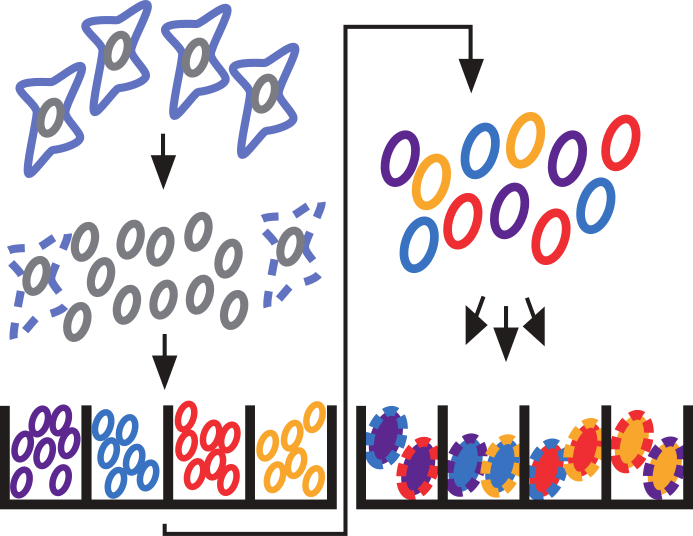
\includegraphics[width=\textwidth]{./ims/cusanovich2015.png}
\end{minipage}\hfill
\begin{minipage}[]{0.45\textwidth}
	\captionsetup{margin={18pt,0pt}, labelfont=bf}
	\caption[Single-cell combinatorial indexing]{\textbf{\Acrlong{sci}.} A suspension of nuclei is equally distributed into wells where they undergo a well-specific barcoding reaction. The nuclei are then pooled and redistributed into a second array of wells, where a second barcode is appended to the first. The majority of nuclei undergo a unique barcoding trajectory, each receiving a unique cellular index that is later used to demultiplex the resulting libraries after sequencing. Adapted from \cite{cusanovich2015}}
	\label{fig:cusanovich2015}
\end{minipage}
\end{figure}

The \acrshort{sci} approach was first used in \citeauthor{cusanovich2015}'s \acrfull{sciatac-seq} method \citep{cusanovich2015}. In \acrshort{sciatac-seq}, a population of {\textasciitilde}2000 nuclei is distributed equally into 96 microwells. Here, the nuclei undergo tagmentation with a well-specific custom Tn5 transposase which carries a well-specific barcode. This step results in a chromatin library of which the fragments are tagged with a first barcode. The tagmented nuclei are then pooled and redistributed into 96 new wells where they undergo \acrshort{pcr} amplification with a barcoded primer, resulting in single-cell \acrshort{atac-seq} libraries. The protocol was later adapted for to \acrshort{scirna-seq} \citep{cao2017} by performing reverse transcription with well-specific barcodes instead of well-specific Tn5 tagmentation. \acrshort{scirna-seq} starts from either single nuclei or fixed and permeabilised cells. The \acrshort{sci} approach can thus be used for both \acrshort{scatac-seq} an \acrshort{scrna-seq}.\pms

As with the high-throughput droplet-microfluidic methods described in section \ref{sec:lit_dropletmicrofluidics}, the sensitivity of \acrshort{sci}-based protocols is sub-par. \citeauthor{fiers2018} remark that \acrshort{sciatac-seq} retrieves \textasciitilde{}2500 chromatin fragment reads per cell compared to \textasciitilde{}73 000 reads per cell from the \citeauthor{buenrostro2015} \acrshort{scatac-seq} protocol (see section \ref{subsect:lit_fluidigm_c1}) \citep{fiers2018}. This difference can in part be explained by the difference in per-cell sequencing coverage between the two methods.\pms

A major single-cell multiomics breakthrough was made in \citeyear{cao2018} when \citeauthor{cao2018} extracted both \acrshort{rna-seq} and \acrshort{atac-seq} data from the same nucleus using a \acrshort{sci}-based approach \citep{cao2018}. The method, called \acrfull{sci-car}, simultaneously barcodes the \acrshort{rna} and chromatin content of single nuclei before splitting the sample for both \acrshort{sciatac-seq} and \acrshort{scirna-seq} processing. Since the \acrshort{cdna} and chromatin reads of the same cell share the same barcode, both libraries can be assigned to their cell of origin. An overview is given in figure \ref{fig:cao2018}.\pms

\begin{figure}[ht]
	\centerfloat
	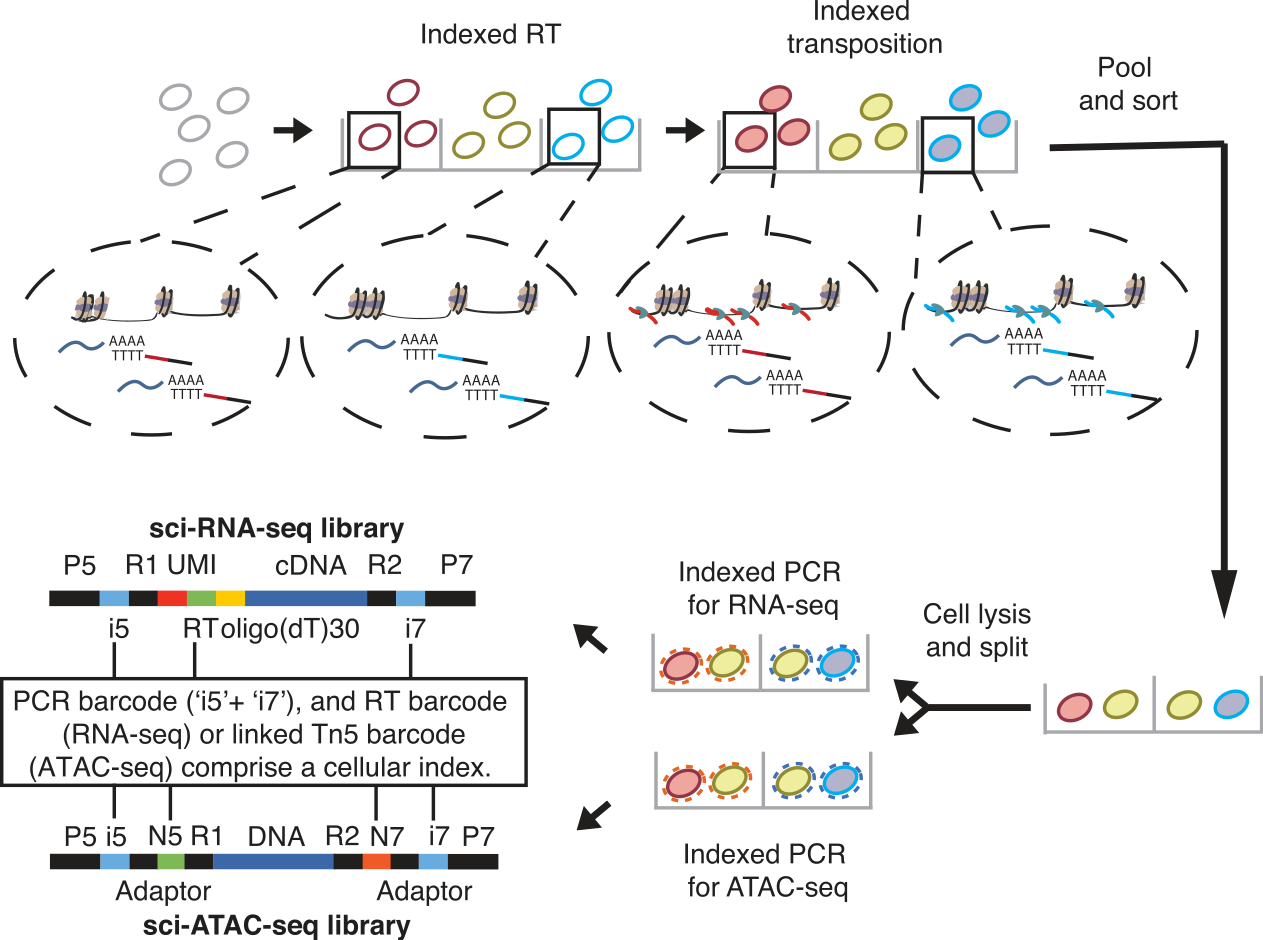
\includegraphics[width=\textwidth]{./ims/shendure2018.png}
	\caption[sci-CAR concept]{\textbf{\Acrshort{sci-car} concept.} Single nuclei are distributed into a 96 well plate at 5 000 nuclei per well, where their \acrshort{rna} content is barcoded by a reverse transcription reaction with a well-specific primer. Next, the nuclei's chromatin content is fragmented and barcoded in the same well by a custom Tn5 carrying a well-specific adapter. In a crucial step, nuclei are first pooled and then \acrshort{facs}-sorted into 576 new wells where the second \acrshort{cdna} strand synthesis occurs. The nuclei are then lysed and the sample is split equally (without pooling) into dedicated portions for subsequent \acrshort{scirna-seq} or \acrshort{sciatac-seq} library generation. Both the \acrshort{rna-seq} and \acrshort{atac-seq} reads can be assigned to the cell of origin based on their barcode combination. Taken from \cite{cao2018}}
	\label{fig:cao2018}
\end{figure}

\Acrshort{sci-car} was applied to extract joint transcriptomic and chromatin accessibility data from 4 825 and 11 296 nuclei, a major increase from other multiomics protocols by e.g. \citet{hou2016} and \citet{clark2018} respectively, which could only be applied to fewer than 100 cells. To date, \acrshort{sci-car} remains the only protocol able to simultaneously profile the transcriptome and chromatin accessibility of high numbers of single cells. Despite the intrinsic value of such datasets in the study of for example gene regulatory networks, \acrshort{sci-car} has not been applied yet by other labs. A hindrance to widespread adoption is the requirement for a custom Tn5 transposase, which is not available commercially. Importantly, \acrshort{sci-car} also discards half of the available cellular material. \Acrshort{sci}-approaches generally require a large number of cells to initiate (10\textsuperscript{5} to 10\textsuperscript{6} cells), and also retrieve about 7-50\% of the sample input, with a high incidence of doublets. A final drawback is that cells/nuclei need to be fixed for \acrshort{sci}, prohibiting the use of fresh samples. Ideally, a multiomic method would barcode and sequence the whole transcriptome and chromatin accessibility profile of cells completely separately. Such a protocol has not been published yet.\pms

\clearpage
\subsection{SPLiT-seq}
\label{subsect:lit_split-seq}
In \citeyear{rosenberg2018}, \citeauthor{rosenberg2018} published \acrfull{split-seq}, a \acrshort{scrna-seq} technique conceptually identical to the Shendure Lab's \acrlong{sci} \acrshort{scrna-seq} \citep{cusanovich2015,rosenberg2018}. Like \acrshort{scirna-seq}, \acrshort{split-seq} indexes fixed cells using successive split/pool in-situ reverse transcription and \acrshort{pcr}. However, the addition of two barcode ligation steps leads to four barcoding opportunities per cell, as opposed to \acrshort{scirna-seq}'s two. This increases overall hands-on time, but allows \acrshort{split-seq} to scale to large numbers of cells more rapidly than \acrshort{scirna-seq}. An overview of the \acrshort{split-seq} barcoding process is given in figure \ref{fig:rosenberg2018}.\pms

\begin{figure}[ht]
\begin{minipage}[]{0.5\textwidth}
	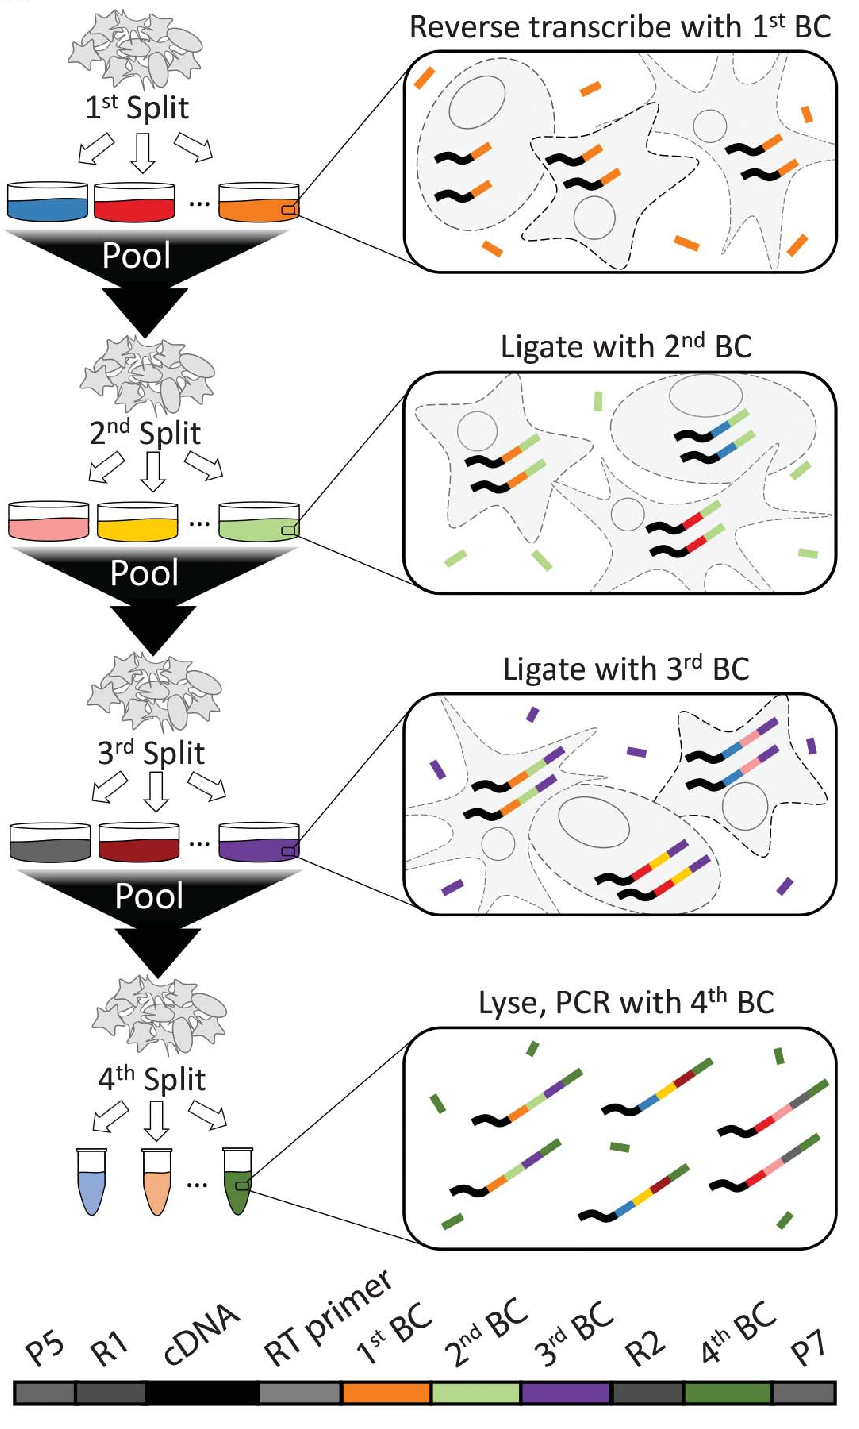
\includegraphics[width=\textwidth]{./ims/rosenberg2018.png}
\end{minipage}\hfill
\begin{minipage}[]{0.45\textwidth}
	\captionsetup{margin={0pt,18pt}, labelfont=bf}
	\caption[Split-pool ligation-based transcriptome sequencing]{\textbf{\Acrfull{split-seq}.} Methanol-fixed and permeabilised cells are split into 48 wells where they undergo in-situ reverse transcription with a well-specific barcode. Two additional barcodes are in-situ ligated to the cellular \acrshort{cdna} libraries in subsequent splitting and pooling steps. The cells are then lysed and a final barcode is introduced in the sequencing library indexing \acrshort{pcr}. Taken from \cite{rosenberg2018}.}
	\label{fig:rosenberg2018}
\end{minipage}
\end{figure}

\acrshort{split-seq}'s main advantage is unprecedented throughput. In theory, \acrshort{split-seq} can barcode more than 6 million cells using just four different microwell plates. It is not unthinkable that future analysis of large cell samples will necessitate experiments of this magnitude. Today, however, the current cost of sequencing and modern computational possibilities prohibit the execution of such ultra-high throughput experiments.

\newpage
\subsection{In-Situ Cellular Indexing: Key Takeaway}
The ultra-high throughput capabilities of combinatorial indexing approaches hold promises for future experiments where 10\textsuperscript{4}-10\textsuperscript{5} cells are analysed. Due to the limits on computation and sequencing technology, such dazzling numbers are unthinkable today. In a sense, the main limiting factor to contemporary single-cell research is by no means the number of cells analysed in a single run. Rather, high-throughput (10\textsuperscript{3}-10\textsuperscript{4} cells), high-sensitivity assays seem to be a more important goal. It is for this reason, combined with the low sensitivity associated with combinatorial indexing and the use of proprietary reagents, that \acrshort{sci} and \acrshort{split-seq} have not been extensively applied outside of their respective labs yet.

\section{Applications of Single-Cell Omics}

\subsection{Cell Typing}

\label{sec:lit_applications}
One of the major applications of single-cell \acrshort{rna-seq} is de-novo cell typing. The \textit{Tabula Muris} is an example of such a large scale effort. The Tabula Muris Consortium sequenced the individual transcriptomes of 55k mouse cells spread over all major organs using 10x Chromium \acrshort{scrna-seq}, and another 45k cells using \acrshort{facs} + \acrshort{smart-seq}2. The resulting cells were computationally separated (figure \ref{fig:schaum2019}) and analysed, identifying several distinct new cell types and transcription factor networks, and revealing previously undiscovered roles of known genes.\pms

\begin{figure}[ht]
	\centerfloat
	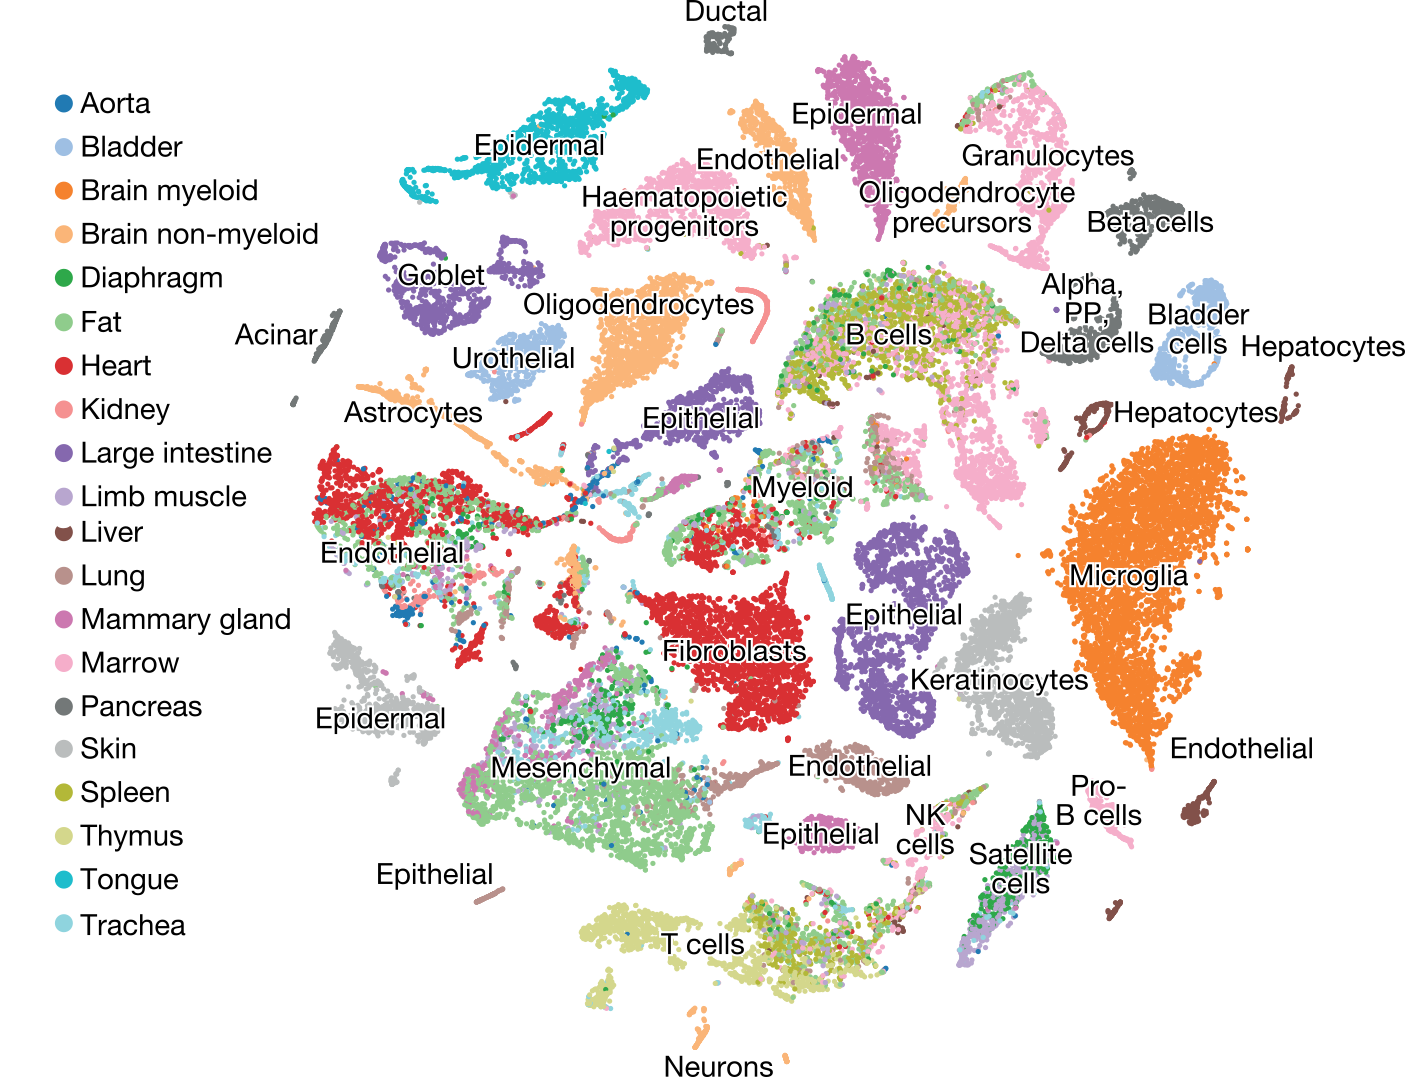
\includegraphics[width=\textwidth]{./ims/test2018.png}
	\caption[Murine cell atlas]{\textbf{Murine cell atlas.} \acrshort{tsne} visualisation of 45k single cell transcriptomes from 20 mouse organs. Taken from \cite{schaum2019}}
	\label{fig:schaum2019}
\end{figure}

Analysing such a large amount of cells spanning over multiple organs allows for direct comparison of the resulting data, but is a major undertaking using the current state of the art technology. The tiered approach employed here, where low sequencing coverage droplet microfluidic methods are used to rapidly form a global picture, and more plate-based methods are used to analyse carefully filtered pre-defined populations at higher sequencing depth, will most likely be the key to undertaking large scale sequencing operations such as these in the future.\pms

\subsection{Development}
During embryogenesis, a single totipotent cell will divide, and its descendants will gradually lose potency and differentiate into the cell types that make up the organism. The acquisition of cell identity, function and morphology is for a large part controlled through differential gene expression \citep{farrell2018}, making high-throughput \acrshort{scrna-seq} a valuable tool in our effort to understand this complex process.\pms

\citeauthor{farrell2018} analysed the individual transcriptomes of 39k zebrafish cells from 12 different embryonic stages using Drop-seq and developed novel computational methods (a combination of URD and Seurat) to map the differentiation process of 25 cell lineages during embryonic development (figure \ref{fig:farrell2018}). The tips of the resulting tree corresponded to previously known cell types in terms of marker gene expression, and much of what was already known about embryonic development was reflected in the tree's branching structure.\pms

\begin{figure}[ht]
	\begin{minipage}[]{0.70\textwidth}
		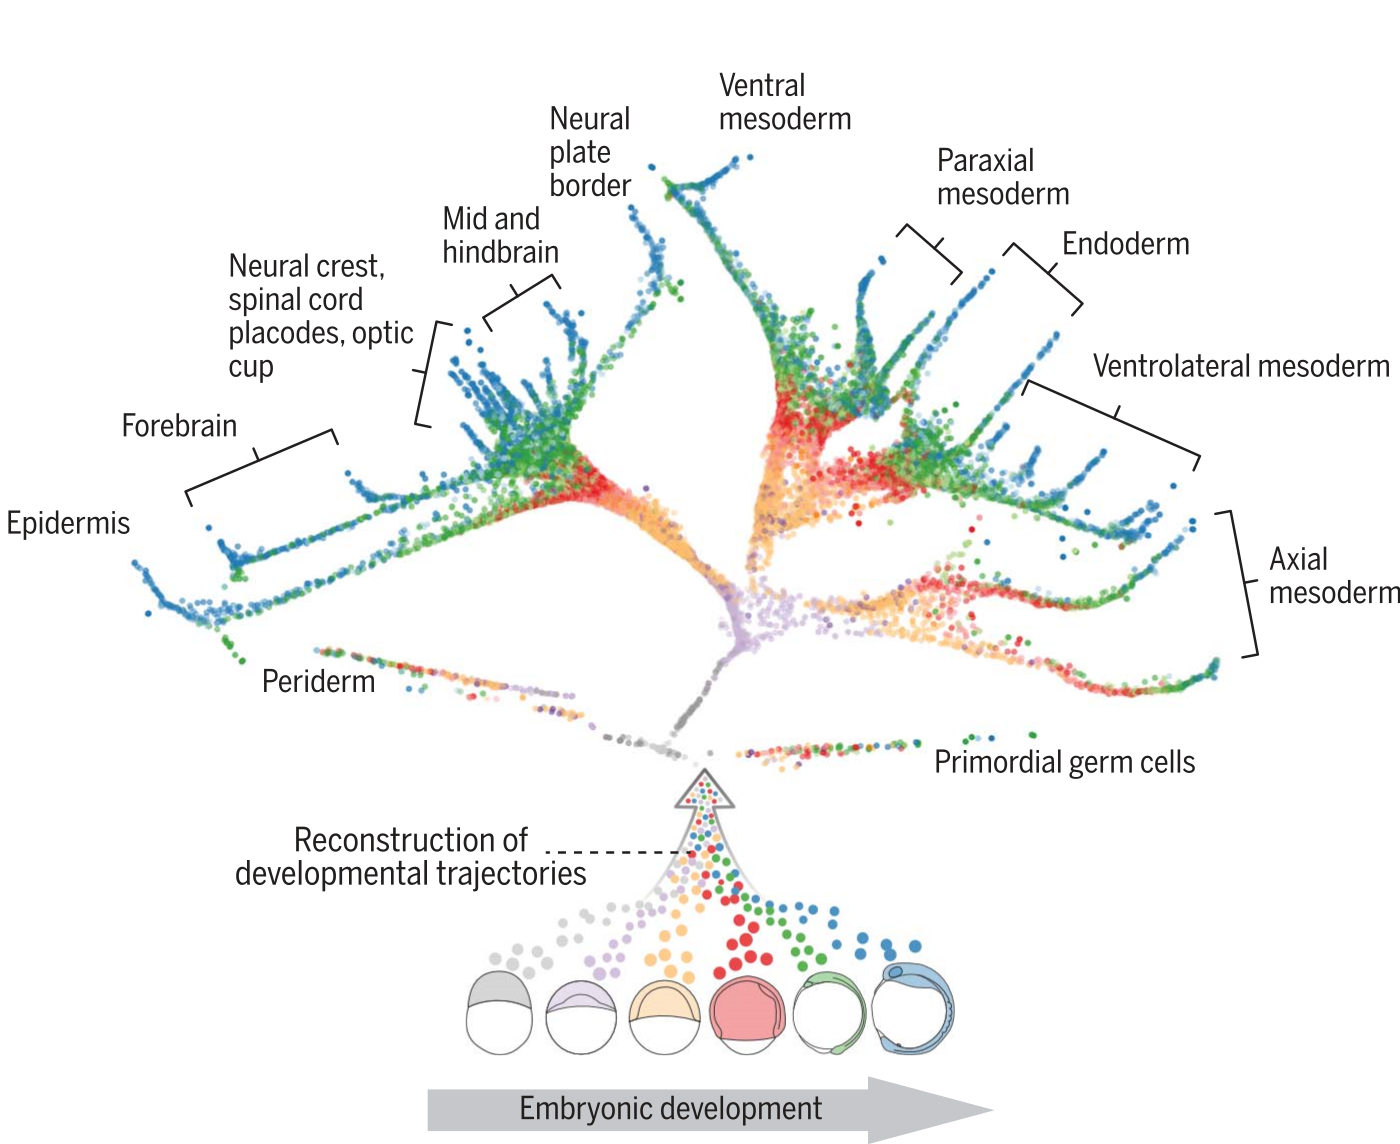
\includegraphics[width=\textwidth]{./ims/farrell2018.png}
	\end{minipage}\hfill
	\begin{minipage}[]{0.25\textwidth}
		\captionsetup{margin={0pt,0pt}, labelfont=bf}
		\caption[Developmental trajectories in Zebrafish embryogenesis]{\textbf{Developmental trajectories in Zebrafish.} Taken from \cite{farrell2018}}
		\label{fig:farrell2018}
	\end{minipage}
\end{figure}

In addition to agreement with the canonical embryological knowledge, the systems biology approach revealed new candidate regulators of the differentiation process and how the spatial organisation of the developing embryo may be decided earlier in development than previously thought. Importantly, the computational framework developed by \citeauthor{farrell2018} can be used for the reconstruction of the developmental trajectories of other biological model organisms.\pms

Another new computational tool was pioneered by \citeauthor{lamanno2018} in \citeyear{lamanno2018}, who realised that the time derivative of gene expression profiles across samples taken on multiple time points could be inferred from the identity of unspliced and mature \acrshort{mrna} transcripts. They found that in several open-access single-cell \acrshort{rna-seq} datasets from samples taken at different time points, the population of immature \acrshort{mrna} transcripts was present as mature transcripts at the next time point. \citeauthor{lamanno2018} then used this information to project the developmental flow on regular \acrshort{tsne} plots (figure \ref{fig:lamanno2018}).\pms

\begin{wrapfigure}{L}{0.50\textwidth}
	\centering
	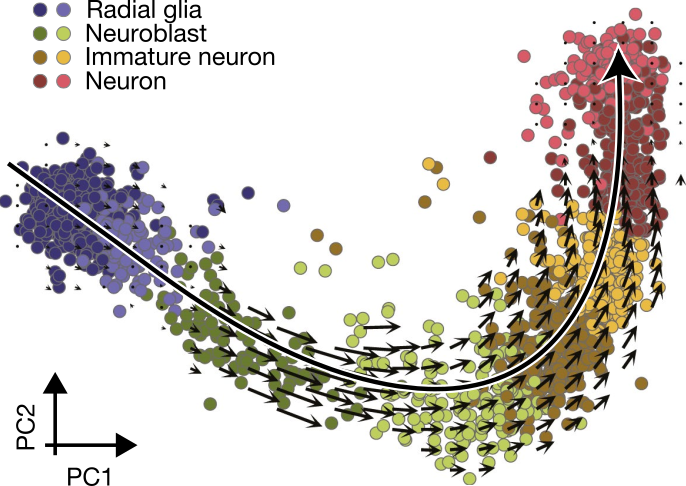
\includegraphics[width=0.45\textwidth]{./ims/lamanno2018.png}
	\captionsetup{margin={0pt,6pt},labelfont=bf}
	\caption[RNA velocity in human neurogenesis]{\textbf{\acrshort{rna} velocity in human neurogenesis.} Taken from \cite{lamanno2018}}
	\label{fig:lamanno2018}
	\vspace{20pt}
\end{wrapfigure}

As this method was first performed on previously published data, this publication proves that new information can often be extracted from the datasets generated by single-cell sequencing experiments when approaching them from a different angle. When a sequencing dataset is generated, it exists permanently as a vector space in which future in-silico "experiments" can be performed, as opposed to classical experiments where samples may have a limited lifetime and interrogating the same sample at a later time point may be difficult. In the future, we may thus see more examples where discoveries are made in older datasets thought to be exhausted of information.\pms

\clearpage
\subsection{Disease}
\begin{wrapfigure}{R}{0.45\textwidth}
	\centering
	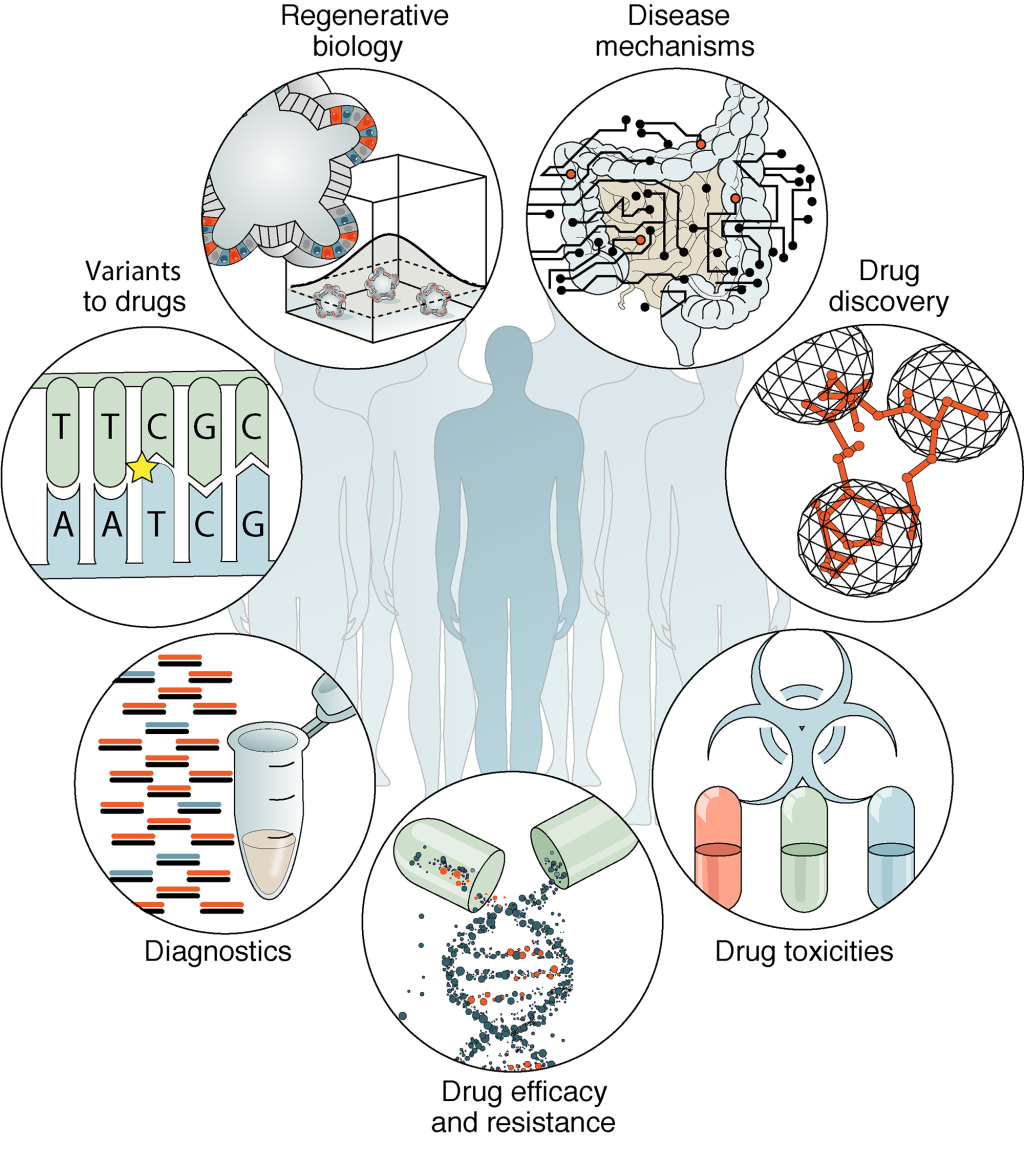
\includegraphics[width=0.40\textwidth]{./ims/hca2017.png}
	\captionsetup{margin={6pt,0pt},labelfont=bf}
	\caption[Impact areas of the Human Cell Atlas]{\textbf{Impact areas of the \acrlong{hca}.} Taken from \cite{hca2017}}
	\label{fig:hca2017}
	\vspace{-20pt}
\end{wrapfigure}

The final application of single cell technology, and its main accelerator today, is human medicine. Several areas of medicine will directly benefit from single-cell resolution data, notably those where cell diversity is most impactful - such as cancer and brain disease. Today's leading effort in pushing single-cell technology to applications in medicine is the \acrfull{hca} \citep{regev2017}. This project, which aims to approach the Human Genome Project in magnitude and scope, aims to comprehensively map all cells present in the human body. Such an atlas could be used as a reference for patient sample comparisons and help understand the cellular mechanisms behind disease. Figure \ref{fig:hca2017} shows the key impact aims of the \acrshort{hca}.\pms

A major application of the \acrshort{hca} will be targeted drug discovery. Comparing the genetic profile of healthy cell samples to the reference cell atlas would provide leads for possible new drugs. Single-cell experiments could also be used to compare in-vitro generated cell cultures with the reference profile of the human tissue they attempt to mimic, accelerating the development of engineered tissues for regenerative medicine. The project's first draft, published in \citeyear{hca2017}, profiles a subset of cells from the tissues and organs that hold the most promise for immediate application. The first draft includes 'only' 30 to 100 million cells, a fraction of the projected 10 billion for the final atlas \citep{hca2017}. \pms

\clearpage
\section{Single-cell Omics: Current Progress and Future Perspectives}
As shown in the previous sections, the past few years have seen an explosion in single-cell research and technology. Single-cell transcriptomics, genomics and epigenomics are already a fact, and proteomics and spatial omics are looming over the horizon. Single cell technology has allowed us to capture snapshots of complex cellular processes such as gene regulation, gene expression, tissue development, and the origins of disease. Even in its infancy, single-cell technology has proven its value in almost every area of biology involving cells. We have uncovered regulatory pathways and mapped the (partial) transcriptome atlases of several model organisms, and are rapidly moving forward to achieving the same in humans. However, much remains to be done. It is painstakingly clear that the vast majority of today's single-cell technology can be further improved upon. Our most cutting-edge high-throughput techniques are able to capture only a small fraction of the information embedded in a single cell, with low reproducibility and high noise levels. Indeed, we are asking much of our bioinformatician colleagues. Equally concerning is how virtually every single-cell technique to date can only interrogate a single omics modality. It is therefore difficult to, for example, systematically relate a cell's transcriptome to its epigenome. The clear-cut next step is therefore to fine-tune existing methods and to move forward to single-cell multi-omics. Extracting information on several omics modalities from the same single cells, at high fidelity \textit{and} close spatial resolution will help us understand the absolute fundamentals of life - and how we may improve it.\pms

% Often, a conscious trade-off is made between sensitivity and throughput. \citeauthor{kalisky2018} suggest a tiered approach: high-throughput, pooled library approaches such as inDrop or \acrshort{split-seq} may be used to systematically analyse large volumes of cells to identify new types or markers. These selected markers or cell-types can then be studied in high-sensitivity assays such as \acrshort{smart-seq}. These methods can profile allele-specific expression, splice isoforms other and full-transcript modalities in single cells and their shed light on their relation to phenotype. The targets established in these increasingly\pms

% These methods can be evaluated using number of criteria, most of which are related to their throughout (price per cell, time per run, number of cells per run) and the quality of the single-cell data they produce (number of transcripts and genese detected per cell, cell multiplet rate). As each cell is destroyed during processing, it is technically impossible to asses technical variation using replicate measurements. One way to overcome this is by spiking the cell lysates with \acrfullpl{ercc}. These sets of spiked-in transcripts are picked up during library preparation, and the extent and profile of their presence in the resulting dataset yields information about the method's sensitivity and possible biases. Another important measure of quality is the average number of genes, and if the method permits, \acrshortpl{umi}, detected per cell. Such approaches cannot be used to compare experiments run on different cell lines or organisms, as differences in cell size and general stochasticity will distort the comparison.\pms

% Here, we show an aggregate of benchmark datasets generated in several comparative experiments \citep{wu2014, ziegenhain2017, zhang2019}. An array of parameters is examined for every method.\pms


% \begin{enumerate}
%\item sensitivity: ability to lowly expressed genes
%\item accuracy: how close to true expression profile
%\item precision: reproducibility
%\item throughput: number of cells that can be measured
%\item transcript coverage
%\item multiplexing ability
%\item cell capture ability
%\item price per cell
%\item price of peripherals
% \end{enumerate}


% A number of papers are discussed.
% \begin{enumerate}
%\item \citep{wu2014} "Quantitative assessment of single-cell rnA-sequencing methods"
%\item \citep{ziegenhain2017} "Comparative Analysis of Droplet-Based Ultra-High- Throughput Single-Cell RNA-Seq Systems"
%\item \citep{zhang2019} "Comparative Analysis of Single-Cell RNA Sequencing Methods"
% \end{enumerate}
